\documentclass[twoside]{book}

% Packages required by doxygen
\usepackage{calc}
\usepackage{doxygen}
\usepackage{graphicx}
\usepackage[utf8]{inputenc}
\usepackage{makeidx}
\usepackage{multicol}
\usepackage{multirow}
\usepackage{textcomp}
\usepackage[table]{xcolor}

% Font selection
\usepackage[T1]{fontenc}
\usepackage{mathptmx}
\usepackage[scaled=.90]{helvet}
\usepackage{courier}
\usepackage{amssymb}
\usepackage{sectsty}
\renewcommand{\familydefault}{\sfdefault}
\allsectionsfont{%
  \fontseries{bc}\selectfont%
  \color{darkgray}%
}
\renewcommand{\DoxyLabelFont}{%
  \fontseries{bc}\selectfont%
  \color{darkgray}%
}

% Page & text layout
\usepackage{geometry}
\geometry{%
  a4paper,%
  top=2.5cm,%
  bottom=2.5cm,%
  left=2.5cm,%
  right=2.5cm%
}
\tolerance=750
\hfuzz=15pt
\hbadness=750
\setlength{\emergencystretch}{15pt}
\setlength{\parindent}{0cm}
\setlength{\parskip}{0.2cm}
\makeatletter
\renewcommand{\paragraph}{%
  \@startsection{paragraph}{4}{0ex}{-1.0ex}{1.0ex}{%
    \normalfont\normalsize\bfseries\SS@parafont%
  }%
}
\renewcommand{\subparagraph}{%
  \@startsection{subparagraph}{5}{0ex}{-1.0ex}{1.0ex}{%
    \normalfont\normalsize\bfseries\SS@subparafont%
  }%
}
\makeatother

% Headers & footers
\usepackage{fancyhdr}
\pagestyle{fancyplain}
\fancyhead[LE]{\fancyplain{}{\bfseries\thepage}}
\fancyhead[CE]{\fancyplain{}{}}
\fancyhead[RE]{\fancyplain{}{\bfseries\leftmark}}
\fancyhead[LO]{\fancyplain{}{\bfseries\rightmark}}
\fancyhead[CO]{\fancyplain{}{}}
\fancyhead[RO]{\fancyplain{}{\bfseries\thepage}}
\fancyfoot[LE]{\fancyplain{}{}}
\fancyfoot[CE]{\fancyplain{}{}}
\fancyfoot[RE]{\fancyplain{}{\bfseries\scriptsize Generated on Mon Jul 8 2013 12:32:15 for Canary API by Doxygen }}
\fancyfoot[LO]{\fancyplain{}{\bfseries\scriptsize Generated on Mon Jul 8 2013 12:32:15 for Canary API by Doxygen }}
\fancyfoot[CO]{\fancyplain{}{}}
\fancyfoot[RO]{\fancyplain{}{}}
\renewcommand{\footrulewidth}{0.4pt}
\renewcommand{\chaptermark}[1]{%
  \markboth{#1}{}%
}
\renewcommand{\sectionmark}[1]{%
  \markright{\thesection\ #1}%
}

% Indices & bibliography
\usepackage{natbib}
\usepackage[titles]{tocloft}
\setcounter{tocdepth}{3}
\setcounter{secnumdepth}{5}
\makeindex

% Hyperlinks (required, but should be loaded last)
\usepackage{ifpdf}
\ifpdf
  \usepackage[pdftex,pagebackref=true]{hyperref}
\else
  \usepackage[ps2pdf,pagebackref=true]{hyperref}
\fi
\hypersetup{%
  colorlinks=true,%
  linkcolor=blue,%
  citecolor=blue,%
  unicode%
}

% Custom commands
\newcommand{\clearemptydoublepage}{%
  \newpage{\pagestyle{empty}\cleardoublepage}%
}


%===== C O N T E N T S =====

\begin{document}

% Titlepage & ToC
\hypersetup{pageanchor=false}
\pagenumbering{roman}
\begin{titlepage}
\vspace*{7cm}
\begin{center}%
{\Large Canary A\-P\-I \\[1ex]\large 1.\-0 }\\
\vspace*{1cm}
{\large Generated by Doxygen 1.8.4}\\
\vspace*{0.5cm}
{\small Mon Jul 8 2013 12:32:15}\\
\end{center}
\end{titlepage}
\clearemptydoublepage
\tableofcontents
\clearemptydoublepage
\pagenumbering{arabic}
\hypersetup{pageanchor=true}

%--- Begin generated contents ---
\chapter{Canary\-A\-P\-I}
\label{md_README}
\hypertarget{md_README}{}
Dependencies\-:

Tornado Tornadio2 \-: \href{https://github.com/mrjoes/tornadio2}{\tt https\-://github.\-com/mrjoes/tornadio2} 
\chapter{Namespace Index}
\section{Namespace List}
Here is a list of all documented namespaces with brief descriptions\-:\begin{DoxyCompactList}
\item\contentsline{section}{\hyperlink{namespaceapi}{api} }{\pageref{namespaceapi}}{}
\item\contentsline{section}{\hyperlink{namespace_canary_assets_1_1_device}{Canary\-Assets.\-Device} }{\pageref{namespace_canary_assets_1_1_device}}{}
\item\contentsline{section}{\hyperlink{namespace_canary_assets_1_1_nest}{Canary\-Assets.\-Nest} }{\pageref{namespace_canary_assets_1_1_nest}}{}
\item\contentsline{section}{\hyperlink{namespace_canary_assets_1_1_user}{Canary\-Assets.\-User} }{\pageref{namespace_canary_assets_1_1_user}}{}
\item\contentsline{section}{\hyperlink{namespace_canary_models_1_1_battery}{Canary\-Models.\-Battery} }{\pageref{namespace_canary_models_1_1_battery}}{}
\item\contentsline{section}{\hyperlink{namespace_canary_models_1_1_c_o}{Canary\-Models.\-C\-O} }{\pageref{namespace_canary_models_1_1_c_o}}{}
\item\contentsline{section}{\hyperlink{namespace_canary_models_1_1_c_o2}{Canary\-Models.\-C\-O2} }{\pageref{namespace_canary_models_1_1_c_o2}}{}
\item\contentsline{section}{\hyperlink{namespace_canary_models_1_1_nearby_hazard}{Canary\-Models.\-Nearby\-Hazard} }{\pageref{namespace_canary_models_1_1_nearby_hazard}}{}
\item\contentsline{section}{\hyperlink{namespace_canary_models_1_1_n_o2}{Canary\-Models.\-N\-O2} }{\pageref{namespace_canary_models_1_1_n_o2}}{}
\item\contentsline{section}{\hyperlink{namespace_canary_models_1_1_outdoor_quality}{Canary\-Models.\-Outdoor\-Quality} }{\pageref{namespace_canary_models_1_1_outdoor_quality}}{}
\item\contentsline{section}{\hyperlink{namespace_canary_models_1_1_p_m10}{Canary\-Models.\-P\-M10} }{\pageref{namespace_canary_models_1_1_p_m10}}{}
\item\contentsline{section}{\hyperlink{namespace_canary_models_1_1_p_m2__5}{Canary\-Models.\-P\-M2\-\_\-5} }{\pageref{namespace_canary_models_1_1_p_m2__5}}{}
\item\contentsline{section}{\hyperlink{namespace_canary_models_1_1_smoke}{Canary\-Models.\-Smoke} }{\pageref{namespace_canary_models_1_1_smoke}}{}
\item\contentsline{section}{\hyperlink{namespace_canary_models_1_1_temperature}{Canary\-Models.\-Temperature} }{\pageref{namespace_canary_models_1_1_temperature}}{}
\item\contentsline{section}{\hyperlink{namespace_canary_utils_1_1_authentication}{Canary\-Utils.\-Authentication} }{\pageref{namespace_canary_utils_1_1_authentication}}{}
\end{DoxyCompactList}

\chapter{Hierarchical Index}
\section{Class Hierarchy}
This inheritance list is sorted roughly, but not completely, alphabetically\-:\begin{DoxyCompactList}
\item \contentsline{section}{Canary\-Assets.\-Asset.\-Asset}{\pageref{class_canary_assets_1_1_asset_1_1_asset}}{}
\item \contentsline{section}{api.\-Canary\-Call}{\pageref{classapi_1_1_canary_call}}{}
\item \contentsline{section}{Canary\-Models.\-Model.\-Model}{\pageref{class_canary_models_1_1_model_1_1_model}}{}
\item Request\-Handler\begin{DoxyCompactList}
\item \contentsline{section}{api.\-Communicator}{\pageref{classapi_1_1_communicator}}{}
\item \contentsline{section}{api.\-Device}{\pageref{classapi_1_1_device}}{}
\item \contentsline{section}{api.\-Devices}{\pageref{classapi_1_1_devices}}{}
\item \contentsline{section}{api.\-Nest}{\pageref{classapi_1_1_nest}}{}
\item \contentsline{section}{api.\-Nests}{\pageref{classapi_1_1_nests}}{}
\item \contentsline{section}{api.\-Ping}{\pageref{classapi_1_1_ping}}{}
\item \contentsline{section}{api.\-User}{\pageref{classapi_1_1_user}}{}
\item \contentsline{section}{api.\-Users}{\pageref{classapi_1_1_users}}{}
\item \contentsline{section}{hailingfrequency.\-Hailing\-Frequency\-Handler}{\pageref{classhailingfrequency_1_1_hailing_frequency_handler}}{}
\item \contentsline{section}{hailingfrequency.\-Socket\-I\-O\-Handler}{\pageref{classhailingfrequency_1_1_socket_i_o_handler}}{}
\end{DoxyCompactList}
\item Socket\-Connection\begin{DoxyCompactList}
\item \contentsline{section}{hailingfrequency.\-Hailing\-Frequency}{\pageref{classhailingfrequency_1_1_hailing_frequency}}{}
\item \contentsline{section}{hailingfrequency.\-Router}{\pageref{classhailingfrequency_1_1_router}}{}
\end{DoxyCompactList}
\item Asset\begin{DoxyCompactList}
\item \contentsline{section}{Canary\-Assets.\-Device.\-Device}{\pageref{class_canary_assets_1_1_device_1_1_device}}{}
\item \contentsline{section}{Canary\-Assets.\-Nest.\-Nest}{\pageref{class_canary_assets_1_1_nest_1_1_nest}}{}
\item \contentsline{section}{Canary\-Assets.\-User.\-User}{\pageref{class_canary_assets_1_1_user_1_1_user}}{}
\end{DoxyCompactList}
\item Model\begin{DoxyCompactList}
\item \contentsline{section}{Canary\-Models.\-Battery.\-Battery}{\pageref{class_canary_models_1_1_battery_1_1_battery}}{}
\item \contentsline{section}{Canary\-Models.\-C\-O2.\-C\-O2}{\pageref{class_canary_models_1_1_c_o2_1_1_c_o2}}{}
\item \contentsline{section}{Canary\-Models.\-C\-O.\-C\-O}{\pageref{class_canary_models_1_1_c_o_1_1_c_o}}{}
\item \contentsline{section}{Canary\-Models.\-Nearby\-Hazard.\-Nearby\-Hazard}{\pageref{class_canary_models_1_1_nearby_hazard_1_1_nearby_hazard}}{}
\item \contentsline{section}{Canary\-Models.\-N\-O2.\-N\-O2}{\pageref{class_canary_models_1_1_n_o2_1_1_n_o2}}{}
\item \contentsline{section}{Canary\-Models.\-Outdoor\-Quality.\-Outdoor\-Quality}{\pageref{class_canary_models_1_1_outdoor_quality_1_1_outdoor_quality}}{}
\item \contentsline{section}{Canary\-Models.\-P\-M10.\-P\-M10}{\pageref{class_canary_models_1_1_p_m10_1_1_p_m10}}{}
\item \contentsline{section}{Canary\-Models.\-P\-M2\-\_\-5.\-P\-M2\-\_\-5}{\pageref{class_canary_models_1_1_p_m2__5_1_1_p_m2__5}}{}
\item \contentsline{section}{Canary\-Models.\-Smoke.\-Smoke}{\pageref{class_canary_models_1_1_smoke_1_1_smoke}}{}
\item \contentsline{section}{Canary\-Models.\-Temperature.\-Temperature}{\pageref{class_canary_models_1_1_temperature_1_1_temperature}}{}
\end{DoxyCompactList}
\end{DoxyCompactList}

\chapter{Class Index}
\section{Class List}
Here are the classes, structs, unions and interfaces with brief descriptions\-:\begin{DoxyCompactList}
\item\contentsline{section}{\hyperlink{classasset_1_1_asset}{asset.\-Asset} }{\pageref{classasset_1_1_asset}}{}
\item\contentsline{section}{\hyperlink{classapi_1_1_canary_call}{api.\-Canary\-Call} }{\pageref{classapi_1_1_canary_call}}{}
\item\contentsline{section}{\hyperlink{classapi_1_1_communicator}{api.\-Communicator} }{\pageref{classapi_1_1_communicator}}{}
\item\contentsline{section}{\hyperlink{classdevice_1_1_device}{device.\-Device} }{\pageref{classdevice_1_1_device}}{}
\item\contentsline{section}{\hyperlink{classapi_1_1_device}{api.\-Device} }{\pageref{classapi_1_1_device}}{}
\item\contentsline{section}{\hyperlink{classapi_1_1_devices}{api.\-Devices} }{\pageref{classapi_1_1_devices}}{}
\item\contentsline{section}{\hyperlink{classhailingfrequency_1_1_hailing_frequency}{hailingfrequency.\-Hailing\-Frequency} }{\pageref{classhailingfrequency_1_1_hailing_frequency}}{}
\item\contentsline{section}{\hyperlink{classhailingfrequency_1_1_hailing_frequency_handler}{hailingfrequency.\-Hailing\-Frequency\-Handler} }{\pageref{classhailingfrequency_1_1_hailing_frequency_handler}}{}
\item\contentsline{section}{\hyperlink{classapi_1_1_nest}{api.\-Nest} }{\pageref{classapi_1_1_nest}}{}
\item\contentsline{section}{\hyperlink{classnest_1_1_nest}{nest.\-Nest} }{\pageref{classnest_1_1_nest}}{}
\item\contentsline{section}{\hyperlink{classapi_1_1_nests}{api.\-Nests} }{\pageref{classapi_1_1_nests}}{}
\item\contentsline{section}{\hyperlink{classapi_1_1_ping}{api.\-Ping} }{\pageref{classapi_1_1_ping}}{}
\item\contentsline{section}{\hyperlink{classhailingfrequency_1_1_router}{hailingfrequency.\-Router} }{\pageref{classhailingfrequency_1_1_router}}{}
\item\contentsline{section}{\hyperlink{classhailingfrequency_1_1_socket_i_o_handler}{hailingfrequency.\-Socket\-I\-O\-Handler} }{\pageref{classhailingfrequency_1_1_socket_i_o_handler}}{}
\item\contentsline{section}{\hyperlink{classuser_1_1_user}{user.\-User} }{\pageref{classuser_1_1_user}}{}
\item\contentsline{section}{\hyperlink{classapi_1_1_user}{api.\-User} }{\pageref{classapi_1_1_user}}{}
\item\contentsline{section}{\hyperlink{classapi_1_1_users}{api.\-Users} }{\pageref{classapi_1_1_users}}{}
\end{DoxyCompactList}

\chapter{Namespace Documentation}
\hypertarget{namespaceapi}{\section{api Namespace Reference}
\label{namespaceapi}\index{api@{api}}
}
\subsection*{Classes}
\begin{DoxyCompactItemize}
\item 
class \hyperlink{classapi_1_1_canary_call}{Canary\-Call}
\item 
class \hyperlink{classapi_1_1_users}{Users}
\item 
class \hyperlink{classapi_1_1_user}{User}
\item 
class \hyperlink{classapi_1_1_nests}{Nests}
\item 
class \hyperlink{classapi_1_1_nest}{Nest}
\item 
class \hyperlink{classapi_1_1_devices}{Devices}
\item 
class \hyperlink{classapi_1_1_device}{Device}
\item 
class \hyperlink{classapi_1_1_ping}{Ping}
\item 
class \hyperlink{classapi_1_1_status}{Status}
\item 
class \hyperlink{classapi_1_1_communicator}{Communicator}
\end{DoxyCompactItemize}
\subsection*{Variables}
\begin{DoxyCompactItemize}
\item 
tuple {\bfseries api}
\item 
\hypertarget{namespaceapi_a1125afafaabf4d39e0f633946f62eecd}{tuple {\bfseries http\-\_\-server} = tornado.\-httpserver.\-H\-T\-T\-P\-Server(api)}\label{namespaceapi_a1125afafaabf4d39e0f633946f62eecd}

\end{DoxyCompactItemize}


\subsection{Detailed Description}
\begin{DoxyVerb}@package Canary.Api

The main API for the cloud-based service.
\end{DoxyVerb}
 

\subsection{Variable Documentation}
\hypertarget{namespaceapi_a5697ea202319f894facccacf78d93e89}{\index{api@{api}!api@{api}}
\index{api@{api}!api@{api}}
\subsubsection[{api}]{\setlength{\rightskip}{0pt plus 5cm}tuple api.\-api}}\label{namespaceapi_a5697ea202319f894facccacf78d93e89}
{\bfseries Initial value\-:}
\begin{DoxyCode}
1 = tornado.web.Application([
2     (\textcolor{stringliteral}{r"/users/"}, Users),
3     (\textcolor{stringliteral}{r"/user/(.*)/"}, User, dict(userId = \textcolor{keywordtype}{None})),
4     (\textcolor{stringliteral}{r"/nests/"}, Nests),
5     (\textcolor{stringliteral}{r"/nest/(.*)/"}, Nest, dict(nestId = \textcolor{keywordtype}{None})),
6     (\textcolor{stringliteral}{r"/nest/(.*)/communicator/"}, Communicator, dict(nestId = \textcolor{keywordtype}{None})),
7     (\textcolor{stringliteral}{r"/devices/"}, Devices),
8     (\textcolor{stringliteral}{r"/device/(.*)/"}, Device, dict(deviceId = \textcolor{keywordtype}{None})),
9     (\textcolor{stringliteral}{r"/ping/(.*)/(.*)/"}, Ping, dict(entityId = \textcolor{keywordtype}{None}, action = \textcolor{keywordtype}{None})),
10     (\textcolor{stringliteral}{r"/status/(.*)/(.*)/"}, Status, dict(entityId = \textcolor{keywordtype}{None}, status = \textcolor{keywordtype}{None})),
11     
12     (\textcolor{stringliteral}{r"/docs/(.*)"}, tornado.web.StaticFileHandler, \{\textcolor{stringliteral}{'path'}: globals.docs\_path\}),    \textcolor{comment}{# helpers; remove in
       production}
13     (\textcolor{stringliteral}{r"/communicator/"}, HailingFrequencyHandler),
14     (\textcolor{stringliteral}{r"/js/socket.io.js"}, SocketIOHandler)
15 ])
\end{DoxyCode}

\hypertarget{namespace_canary_assets_1_1_device}{\section{Canary\-Assets.\-Device Namespace Reference}
\label{namespace_canary_assets_1_1_device}\index{Canary\-Assets.\-Device@{Canary\-Assets.\-Device}}
}
\subsection*{Classes}
\begin{DoxyCompactItemize}
\item 
class \hyperlink{class_canary_assets_1_1_device_1_1_device}{Device}
\end{DoxyCompactItemize}
\subsection*{Variables}
\begin{DoxyCompactItemize}
\item 
dictionary {\bfseries status}
\end{DoxyCompactItemize}


\subsection{Detailed Description}
\begin{DoxyVerb}@package Canary.Asset.Device

Device is a subclass of Asset
\end{DoxyVerb}
 

\subsection{Variable Documentation}
\hypertarget{namespace_canary_assets_1_1_device_af7b2d21f7ba7ccc8ef1352819b9e637d}{\index{Canary\-Assets\-::\-Device@{Canary\-Assets\-::\-Device}!status@{status}}
\index{status@{status}!CanaryAssets::Device@{Canary\-Assets\-::\-Device}}
\subsubsection[{status}]{\setlength{\rightskip}{0pt plus 5cm}dictionary Canary\-Assets.\-Device.\-status}}\label{namespace_canary_assets_1_1_device_af7b2d21f7ba7ccc8ef1352819b9e637d}
{\bfseries Initial value\-:}
\begin{DoxyCode}
1 = \{
2     \textcolor{stringliteral}{'smoke'}: \hyperlink{class_canary_models_1_1_smoke_1_1_smoke}{Smoke}(),
3     \textcolor{stringliteral}{'co'}: \hyperlink{class_canary_models_1_1_c_o_1_1_c_o}{CO}(),
4     \textcolor{stringliteral}{'no2'}: \hyperlink{class_canary_models_1_1_n_o2_1_1_n_o2}{NO2}(),
5     \textcolor{stringliteral}{'pm2\_5'} : \hyperlink{class_canary_models_1_1_p_m2__5_1_1_p_m2__5}{PM2\_5}(),
6     \textcolor{stringliteral}{'pm10'}: \hyperlink{class_canary_models_1_1_p_m10_1_1_p_m10}{PM10}(),
7     \textcolor{stringliteral}{'co2'}: \hyperlink{class_canary_models_1_1_c_o2_1_1_c_o2}{CO2}(),
8     \textcolor{stringliteral}{'temperature'}: \hyperlink{class_canary_models_1_1_temperature_1_1_temperature}{Temperature}(),
9     \textcolor{stringliteral}{'battery'}: \hyperlink{class_canary_models_1_1_battery_1_1_battery}{Battery}()
10 \}
\end{DoxyCode}

\hypertarget{namespace_canary_assets_1_1_nest}{\section{Canary\-Assets.\-Nest Namespace Reference}
\label{namespace_canary_assets_1_1_nest}\index{Canary\-Assets.\-Nest@{Canary\-Assets.\-Nest}}
}
\subsection*{Classes}
\begin{DoxyCompactItemize}
\item 
class \hyperlink{class_canary_assets_1_1_nest_1_1_nest}{Nest}
\end{DoxyCompactItemize}
\subsection*{Variables}
\begin{DoxyCompactItemize}
\item 
\hypertarget{namespace_canary_assets_1_1_nest_a861c75fd638182e19205052a80b368db}{tuple {\bfseries owner} = User()}\label{namespace_canary_assets_1_1_nest_a861c75fd638182e19205052a80b368db}

\item 
\hypertarget{namespace_canary_assets_1_1_nest_a2e64931a173179de2479254126544527}{list {\bfseries members} = \mbox{[}$\,$\mbox{]}}\label{namespace_canary_assets_1_1_nest_a2e64931a173179de2479254126544527}

\item 
\hypertarget{namespace_canary_assets_1_1_nest_ad01b5076589d0887e80c5bfc0faf0cf5}{list {\bfseries devices} = \mbox{[}$\,$\mbox{]}}\label{namespace_canary_assets_1_1_nest_ad01b5076589d0887e80c5bfc0faf0cf5}

\item 
dictionary {\bfseries quality}
\end{DoxyCompactItemize}


\subsection{Detailed Description}
\begin{DoxyVerb}@package Canary.Asset.Nest

Nest is a subclass of Asset
\end{DoxyVerb}
 

\subsection{Variable Documentation}
\hypertarget{namespace_canary_assets_1_1_nest_ab47513933198fdd0489b9ad3bdb169b0}{\index{Canary\-Assets\-::\-Nest@{Canary\-Assets\-::\-Nest}!quality@{quality}}
\index{quality@{quality}!CanaryAssets::Nest@{Canary\-Assets\-::\-Nest}}
\subsubsection[{quality}]{\setlength{\rightskip}{0pt plus 5cm}dictionary Canary\-Assets.\-Nest.\-quality}}\label{namespace_canary_assets_1_1_nest_ab47513933198fdd0489b9ad3bdb169b0}
{\bfseries Initial value\-:}
\begin{DoxyCode}
1 = \{
2     \textcolor{stringliteral}{'outdoor'}: OutdoorQuality(),
3     \textcolor{stringliteral}{'nearby\_hazards'}: []
4 \}
\end{DoxyCode}

\hypertarget{namespace_canary_assets_1_1_user}{\section{Canary\-Assets.\-User Namespace Reference}
\label{namespace_canary_assets_1_1_user}\index{Canary\-Assets.\-User@{Canary\-Assets.\-User}}
}
\subsection*{Classes}
\begin{DoxyCompactItemize}
\item 
class \hyperlink{class_canary_assets_1_1_user_1_1_user}{User}
\end{DoxyCompactItemize}
\subsection*{Variables}
\begin{DoxyCompactItemize}
\item 
\hypertarget{namespace_canary_assets_1_1_user_a663486349c21a6ce89e2418d32bd95a5}{list {\bfseries nests} = \mbox{[}$\,$\mbox{]}}\label{namespace_canary_assets_1_1_user_a663486349c21a6ce89e2418d32bd95a5}

\end{DoxyCompactItemize}


\subsection{Detailed Description}
\begin{DoxyVerb}@package Canary.Asset.User

User is a subclass of Asset
\end{DoxyVerb}
 
\hypertarget{namespace_canary_models_1_1_battery}{\section{Canary\-Models.\-Battery Namespace Reference}
\label{namespace_canary_models_1_1_battery}\index{Canary\-Models.\-Battery@{Canary\-Models.\-Battery}}
}
\subsection*{Classes}
\begin{DoxyCompactItemize}
\item 
class \hyperlink{class_canary_models_1_1_battery_1_1_battery}{Battery}
\end{DoxyCompactItemize}


\subsection{Detailed Description}
\begin{DoxyVerb}@package Canary.Model.Battery

Battery is a subclass of Model
\end{DoxyVerb}
 
\hypertarget{namespace_canary_models_1_1_c_o}{\section{Canary\-Models.\-C\-O Namespace Reference}
\label{namespace_canary_models_1_1_c_o}\index{Canary\-Models.\-C\-O@{Canary\-Models.\-C\-O}}
}
\subsection*{Classes}
\begin{DoxyCompactItemize}
\item 
class \hyperlink{class_canary_models_1_1_c_o_1_1_c_o}{C\-O}
\end{DoxyCompactItemize}


\subsection{Detailed Description}
\begin{DoxyVerb}@package Canary.Model.CO

CO is a subclass of Model
\end{DoxyVerb}
 
\hypertarget{namespace_canary_models_1_1_c_o2}{\section{Canary\-Models.\-C\-O2 Namespace Reference}
\label{namespace_canary_models_1_1_c_o2}\index{Canary\-Models.\-C\-O2@{Canary\-Models.\-C\-O2}}
}
\subsection*{Classes}
\begin{DoxyCompactItemize}
\item 
class \hyperlink{class_canary_models_1_1_c_o2_1_1_c_o2}{C\-O2}
\end{DoxyCompactItemize}


\subsection{Detailed Description}
\begin{DoxyVerb}@package Canary.Model.CO2

CO2 is a subclass of Model
\end{DoxyVerb}
 
\hypertarget{namespace_canary_models_1_1_nearby_hazard}{\section{Canary\-Models.\-Nearby\-Hazard Namespace Reference}
\label{namespace_canary_models_1_1_nearby_hazard}\index{Canary\-Models.\-Nearby\-Hazard@{Canary\-Models.\-Nearby\-Hazard}}
}
\subsection*{Classes}
\begin{DoxyCompactItemize}
\item 
class \hyperlink{class_canary_models_1_1_nearby_hazard_1_1_nearby_hazard}{Nearby\-Hazard}
\end{DoxyCompactItemize}


\subsection{Detailed Description}
\begin{DoxyVerb}@package Canary.Model.NearbyHazard

NearbyHazard is a subclass of Model
\end{DoxyVerb}
 
\hypertarget{namespace_canary_models_1_1_n_o2}{\section{Canary\-Models.\-N\-O2 Namespace Reference}
\label{namespace_canary_models_1_1_n_o2}\index{Canary\-Models.\-N\-O2@{Canary\-Models.\-N\-O2}}
}
\subsection*{Classes}
\begin{DoxyCompactItemize}
\item 
class \hyperlink{class_canary_models_1_1_n_o2_1_1_n_o2}{N\-O2}
\end{DoxyCompactItemize}


\subsection{Detailed Description}
\begin{DoxyVerb}@package Canary.Model.NO2

NO2 is a subclass of Model
\end{DoxyVerb}
 
\hypertarget{namespace_canary_models_1_1_outdoor_quality}{\section{Canary\-Models.\-Outdoor\-Quality Namespace Reference}
\label{namespace_canary_models_1_1_outdoor_quality}\index{Canary\-Models.\-Outdoor\-Quality@{Canary\-Models.\-Outdoor\-Quality}}
}
\subsection*{Classes}
\begin{DoxyCompactItemize}
\item 
class \hyperlink{class_canary_models_1_1_outdoor_quality_1_1_outdoor_quality}{Outdoor\-Quality}
\end{DoxyCompactItemize}


\subsection{Detailed Description}
\begin{DoxyVerb}@package Canary.Model.OutdoorQuality

OutdoorQuality is a subclass of Model
\end{DoxyVerb}
 
\hypertarget{namespace_canary_models_1_1_p_m10}{\section{Canary\-Models.\-P\-M10 Namespace Reference}
\label{namespace_canary_models_1_1_p_m10}\index{Canary\-Models.\-P\-M10@{Canary\-Models.\-P\-M10}}
}
\subsection*{Classes}
\begin{DoxyCompactItemize}
\item 
class \hyperlink{class_canary_models_1_1_p_m10_1_1_p_m10}{P\-M10}
\end{DoxyCompactItemize}


\subsection{Detailed Description}
\begin{DoxyVerb}@package Canary.Model.PM10

PM10 is a subclass of Model
\end{DoxyVerb}
 
\hypertarget{namespace_canary_models_1_1_p_m2__5}{\section{Canary\-Models.\-P\-M2\-\_\-5 Namespace Reference}
\label{namespace_canary_models_1_1_p_m2__5}\index{Canary\-Models.\-P\-M2\-\_\-5@{Canary\-Models.\-P\-M2\-\_\-5}}
}
\subsection*{Classes}
\begin{DoxyCompactItemize}
\item 
class \hyperlink{class_canary_models_1_1_p_m2__5_1_1_p_m2__5}{P\-M2\-\_\-5}
\end{DoxyCompactItemize}


\subsection{Detailed Description}
\begin{DoxyVerb}@package Canary.Model.PM2_5

PM2_5 is a subclass of Model
\end{DoxyVerb}
 
\hypertarget{namespace_canary_models_1_1_smoke}{\section{Canary\-Models.\-Smoke Namespace Reference}
\label{namespace_canary_models_1_1_smoke}\index{Canary\-Models.\-Smoke@{Canary\-Models.\-Smoke}}
}
\subsection*{Classes}
\begin{DoxyCompactItemize}
\item 
class \hyperlink{class_canary_models_1_1_smoke_1_1_smoke}{Smoke}
\end{DoxyCompactItemize}


\subsection{Detailed Description}
\begin{DoxyVerb}@package Canary.Model.Smoke

Smoke is a subclass of Model
\end{DoxyVerb}
 
\hypertarget{namespace_canary_models_1_1_temperature}{\section{Canary\-Models.\-Temperature Namespace Reference}
\label{namespace_canary_models_1_1_temperature}\index{Canary\-Models.\-Temperature@{Canary\-Models.\-Temperature}}
}
\subsection*{Classes}
\begin{DoxyCompactItemize}
\item 
class \hyperlink{class_canary_models_1_1_temperature_1_1_temperature}{Temperature}
\end{DoxyCompactItemize}


\subsection{Detailed Description}
\begin{DoxyVerb}@package Canary.Model.Temperature

Temperature is a subclass of Model
\end{DoxyVerb}
 
\hypertarget{namespace_canary_utils_1_1_authentication}{\section{Canary\-Utils.\-Authentication Namespace Reference}
\label{namespace_canary_utils_1_1_authentication}\index{Canary\-Utils.\-Authentication@{Canary\-Utils.\-Authentication}}
}
\subsection*{Functions}
\begin{DoxyCompactItemize}
\item 
def \hyperlink{namespace_canary_utils_1_1_authentication_a93d745f2e4d5974bd0d13b19f450c747}{grant\-Access\-To\-Entity}
\end{DoxyCompactItemize}


\subsection{Detailed Description}
\begin{DoxyVerb}@package Canary.Utils.Authentication

Methods available for managing authentication between entities.
\end{DoxyVerb}
 

\subsection{Function Documentation}
\hypertarget{namespace_canary_utils_1_1_authentication_a93d745f2e4d5974bd0d13b19f450c747}{\index{Canary\-Utils\-::\-Authentication@{Canary\-Utils\-::\-Authentication}!grant\-Access\-To\-Entity@{grant\-Access\-To\-Entity}}
\index{grant\-Access\-To\-Entity@{grant\-Access\-To\-Entity}!CanaryUtils::Authentication@{Canary\-Utils\-::\-Authentication}}
\subsubsection[{grant\-Access\-To\-Entity}]{\setlength{\rightskip}{0pt plus 5cm}def Canary\-Utils.\-Authentication.\-grant\-Access\-To\-Entity (
\begin{DoxyParamCaption}
\item[{}]{entity\-\_\-id}
\end{DoxyParamCaption}
)}}\label{namespace_canary_utils_1_1_authentication_a93d745f2e4d5974bd0d13b19f450c747}
\begin{DoxyVerb}Grants access to an entity (User, Device, Nest) to perform protected actions.  The bearer's cookie must contain a key that the entity can recognize.\end{DoxyVerb}
 
\chapter{Class Documentation}
\hypertarget{class_canary_assets_1_1_asset_1_1_asset}{\section{Canary\-Assets.\-Asset.\-Asset Class Reference}
\label{class_canary_assets_1_1_asset_1_1_asset}\index{Canary\-Assets.\-Asset.\-Asset@{Canary\-Assets.\-Asset.\-Asset}}
}
\subsection*{Public Member Functions}
\begin{DoxyCompactItemize}
\item 
\hypertarget{class_canary_assets_1_1_asset_1_1_asset_a86ac77042148b8490907c19e59585002}{def {\bfseries \-\_\-\-\_\-init\-\_\-\-\_\-}}\label{class_canary_assets_1_1_asset_1_1_asset_a86ac77042148b8490907c19e59585002}

\item 
def \hyperlink{class_canary_assets_1_1_asset_1_1_asset_a9b0b6f19f09d50dea75071e5c5af494b}{inflate}
\item 
\hypertarget{class_canary_assets_1_1_asset_1_1_asset_acf5d55e86c096f3319b4265d93e0f1c8}{def {\bfseries emit}}\label{class_canary_assets_1_1_asset_1_1_asset_acf5d55e86c096f3319b4265d93e0f1c8}

\item 
def \hyperlink{class_canary_assets_1_1_asset_1_1_asset_ab5655ab09219eb41b0f4b757f3cc339a}{ping}
\end{DoxyCompactItemize}
\subsection*{Static Public Attributes}
\begin{DoxyCompactItemize}
\item 
\hypertarget{class_canary_assets_1_1_asset_1_1_asset_afb1b09475cec8a2a41237a0678d5ec38}{{\bfseries entity\-Id} = None}\label{class_canary_assets_1_1_asset_1_1_asset_afb1b09475cec8a2a41237a0678d5ec38}

\item 
\hypertarget{class_canary_assets_1_1_asset_1_1_asset_ad262abea1621878cbd0b397f0d54356b}{list {\bfseries accepted\-Keys} = \mbox{[}$\,$\mbox{]}}\label{class_canary_assets_1_1_asset_1_1_asset_ad262abea1621878cbd0b397f0d54356b}

\item 
\hypertarget{class_canary_assets_1_1_asset_1_1_asset_ab425107a364d89337e3545ab54a6fc62}{{\bfseries ping\-Protocol} = None}\label{class_canary_assets_1_1_asset_1_1_asset_ab425107a364d89337e3545ab54a6fc62}

\end{DoxyCompactItemize}


\subsection{Detailed Description}
\begin{DoxyVerb}The Asset superclass encapsulates all entities (Users, Nests, Devices).  Its acceptedKeys indicates which users may have access to its methods.\end{DoxyVerb}
 

\subsection{Member Function Documentation}
\hypertarget{class_canary_assets_1_1_asset_1_1_asset_a9b0b6f19f09d50dea75071e5c5af494b}{\index{Canary\-Assets\-::\-Asset\-::\-Asset@{Canary\-Assets\-::\-Asset\-::\-Asset}!inflate@{inflate}}
\index{inflate@{inflate}!CanaryAssets::Asset::Asset@{Canary\-Assets\-::\-Asset\-::\-Asset}}
\subsubsection[{inflate}]{\setlength{\rightskip}{0pt plus 5cm}def Canary\-Assets.\-Asset.\-Asset.\-inflate (
\begin{DoxyParamCaption}
\item[{}]{self, }
\item[{}]{inflate}
\end{DoxyParamCaption}
)}}\label{class_canary_assets_1_1_asset_1_1_asset_a9b0b6f19f09d50dea75071e5c5af494b}
\begin{DoxyVerb}Populates the Asset from values in the Canary Datastore.\end{DoxyVerb}
 \hypertarget{class_canary_assets_1_1_asset_1_1_asset_ab5655ab09219eb41b0f4b757f3cc339a}{\index{Canary\-Assets\-::\-Asset\-::\-Asset@{Canary\-Assets\-::\-Asset\-::\-Asset}!ping@{ping}}
\index{ping@{ping}!CanaryAssets::Asset::Asset@{Canary\-Assets\-::\-Asset\-::\-Asset}}
\subsubsection[{ping}]{\setlength{\rightskip}{0pt plus 5cm}def Canary\-Assets.\-Asset.\-Asset.\-ping (
\begin{DoxyParamCaption}
\item[{}]{self, }
\item[{}]{message = {\ttfamily None}}
\end{DoxyParamCaption}
)}}\label{class_canary_assets_1_1_asset_1_1_asset_ab5655ab09219eb41b0f4b757f3cc339a}
\begin{DoxyVerb}Pings the asset according to its pingProtocol (Google GCM, iOS Push Notification, or other protocol).\end{DoxyVerb}
 

The documentation for this class was generated from the following file\-:\begin{DoxyCompactItemize}
\item 
Canary\-Assets/Asset.\-py\end{DoxyCompactItemize}

\hypertarget{class_canary_models_1_1_battery_1_1_battery}{\section{Canary\-Models.\-Battery.\-Battery Class Reference}
\label{class_canary_models_1_1_battery_1_1_battery}\index{Canary\-Models.\-Battery.\-Battery@{Canary\-Models.\-Battery.\-Battery}}
}
Inheritance diagram for Canary\-Models.\-Battery.\-Battery\-:\begin{figure}[H]
\begin{center}
\leavevmode
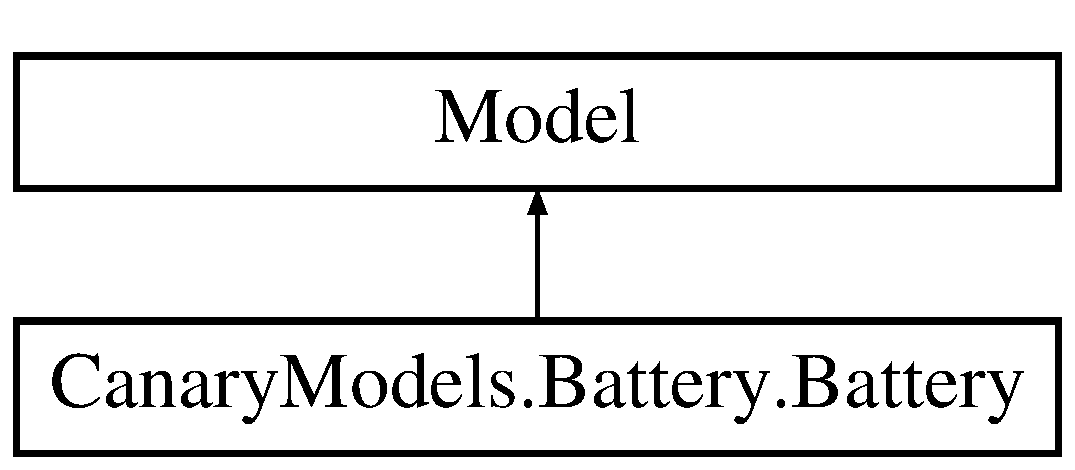
\includegraphics[height=2.000000cm]{class_canary_models_1_1_battery_1_1_battery}
\end{center}
\end{figure}
\subsection*{Public Member Functions}
\begin{DoxyCompactItemize}
\item 
\hypertarget{class_canary_models_1_1_battery_1_1_battery_afa69b07a7d6f918b91650f8f3297584b}{def {\bfseries \-\_\-\-\_\-init\-\_\-\-\_\-}}\label{class_canary_models_1_1_battery_1_1_battery_afa69b07a7d6f918b91650f8f3297584b}

\end{DoxyCompactItemize}


The documentation for this class was generated from the following file\-:\begin{DoxyCompactItemize}
\item 
Canary\-Models/Battery.\-py\end{DoxyCompactItemize}

\hypertarget{classapi_1_1_canary_call}{\section{api.\-Canary\-Call Class Reference}
\label{classapi_1_1_canary_call}\index{api.\-Canary\-Call@{api.\-Canary\-Call}}
}
\subsection*{Public Member Functions}
\begin{DoxyCompactItemize}
\item 
def \hyperlink{classapi_1_1_canary_call_ac588d521c86e5fc5c12f1b3726a64c43}{\-\_\-\-\_\-init\-\_\-\-\_\-}
\item 
def \hyperlink{classapi_1_1_canary_call_a6bfc31d394a2d0009114243d157fe2ed}{emit}
\end{DoxyCompactItemize}
\subsection*{Public Attributes}
\begin{DoxyCompactItemize}
\item 
\hypertarget{classapi_1_1_canary_call_a7e92b23fd21be88cfed022b4a6939040}{{\bfseries result}}\label{classapi_1_1_canary_call_a7e92b23fd21be88cfed022b4a6939040}

\item 
\hypertarget{classapi_1_1_canary_call_a863215d250eb3714a11462265a04c9e3}{{\bfseries data}}\label{classapi_1_1_canary_call_a863215d250eb3714a11462265a04c9e3}

\end{DoxyCompactItemize}


\subsection{Constructor \& Destructor Documentation}
\hypertarget{classapi_1_1_canary_call_ac588d521c86e5fc5c12f1b3726a64c43}{\index{api\-::\-Canary\-Call@{api\-::\-Canary\-Call}!\-\_\-\-\_\-init\-\_\-\-\_\-@{\-\_\-\-\_\-init\-\_\-\-\_\-}}
\index{\-\_\-\-\_\-init\-\_\-\-\_\-@{\-\_\-\-\_\-init\-\_\-\-\_\-}!api::CanaryCall@{api\-::\-Canary\-Call}}
\subsubsection[{\-\_\-\-\_\-init\-\_\-\-\_\-}]{\setlength{\rightskip}{0pt plus 5cm}def api.\-Canary\-Call.\-\_\-\-\_\-init\-\_\-\-\_\- (
\begin{DoxyParamCaption}
\item[{}]{self, }
\item[{}]{result = {\ttfamily None}}
\end{DoxyParamCaption}
)}}\label{classapi_1_1_canary_call_ac588d521c86e5fc5c12f1b3726a64c43}
\begin{DoxyVerb}You may pass CanaryCall an object to set as its data (i.e. the result of a query).  If data is present, the result will automatically be set to 200 (OK).\end{DoxyVerb}
 

\subsection{Member Function Documentation}
\hypertarget{classapi_1_1_canary_call_a6bfc31d394a2d0009114243d157fe2ed}{\index{api\-::\-Canary\-Call@{api\-::\-Canary\-Call}!emit@{emit}}
\index{emit@{emit}!api::CanaryCall@{api\-::\-Canary\-Call}}
\subsubsection[{emit}]{\setlength{\rightskip}{0pt plus 5cm}def api.\-Canary\-Call.\-emit (
\begin{DoxyParamCaption}
\item[{}]{self}
\end{DoxyParamCaption}
)}}\label{classapi_1_1_canary_call_a6bfc31d394a2d0009114243d157fe2ed}
\begin{DoxyVerb}Returns the CanaryCall object as a dict, which can be output as JSON\end{DoxyVerb}
 

The documentation for this class was generated from the following file\-:\begin{DoxyCompactItemize}
\item 
api.\-py\end{DoxyCompactItemize}

\hypertarget{class_canary_models_1_1_c_o_1_1_c_o}{\section{Canary\-Models.\-C\-O.\-C\-O Class Reference}
\label{class_canary_models_1_1_c_o_1_1_c_o}\index{Canary\-Models.\-C\-O.\-C\-O@{Canary\-Models.\-C\-O.\-C\-O}}
}
Inheritance diagram for Canary\-Models.\-C\-O.\-C\-O\-:\begin{figure}[H]
\begin{center}
\leavevmode
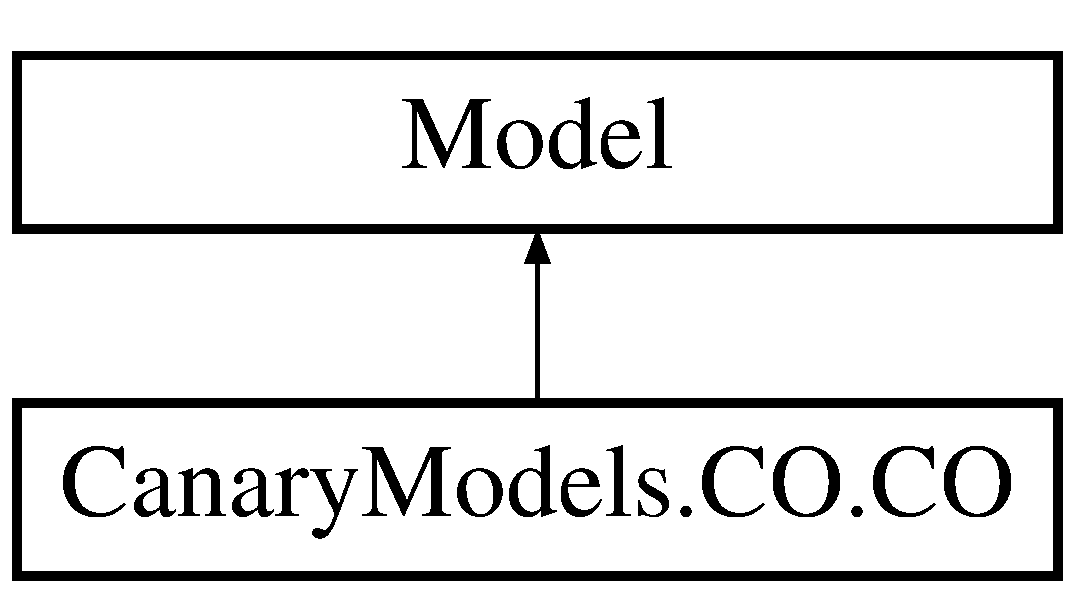
\includegraphics[height=2.000000cm]{class_canary_models_1_1_c_o_1_1_c_o}
\end{center}
\end{figure}
\subsection*{Public Member Functions}
\begin{DoxyCompactItemize}
\item 
\hypertarget{class_canary_models_1_1_c_o_1_1_c_o_af5256a722e68cec80a650442b1e335da}{def {\bfseries \-\_\-\-\_\-init\-\_\-\-\_\-}}\label{class_canary_models_1_1_c_o_1_1_c_o_af5256a722e68cec80a650442b1e335da}

\end{DoxyCompactItemize}


The documentation for this class was generated from the following file\-:\begin{DoxyCompactItemize}
\item 
Canary\-Models/C\-O.\-py\end{DoxyCompactItemize}

\hypertarget{class_canary_models_1_1_c_o2_1_1_c_o2}{\section{Canary\-Models.\-C\-O2.\-C\-O2 Class Reference}
\label{class_canary_models_1_1_c_o2_1_1_c_o2}\index{Canary\-Models.\-C\-O2.\-C\-O2@{Canary\-Models.\-C\-O2.\-C\-O2}}
}
Inheritance diagram for Canary\-Models.\-C\-O2.\-C\-O2\-:\begin{figure}[H]
\begin{center}
\leavevmode
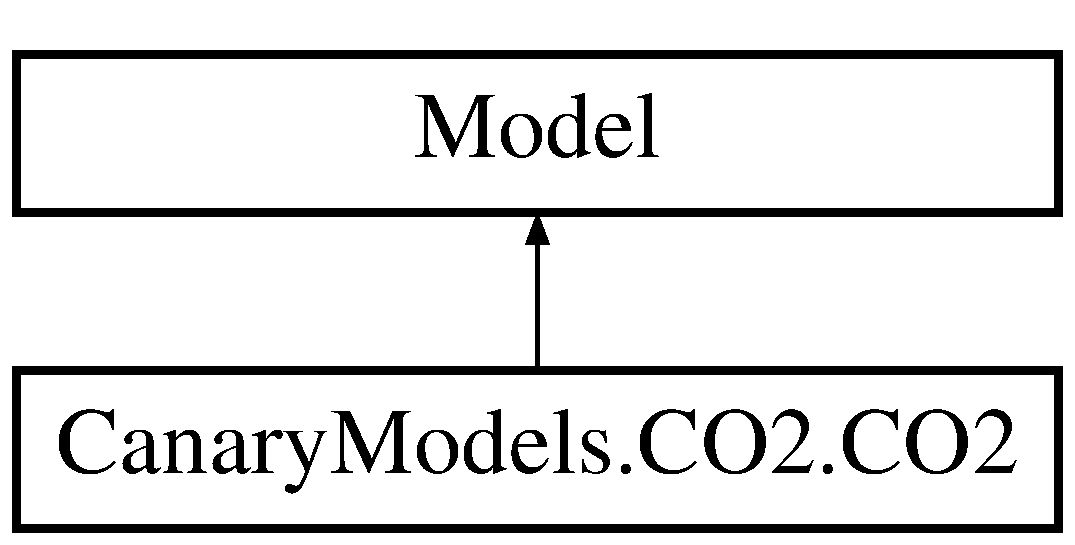
\includegraphics[height=2.000000cm]{class_canary_models_1_1_c_o2_1_1_c_o2}
\end{center}
\end{figure}
\subsection*{Public Member Functions}
\begin{DoxyCompactItemize}
\item 
\hypertarget{class_canary_models_1_1_c_o2_1_1_c_o2_a900e93e586e183f0515f566b08a08af2}{def {\bfseries \-\_\-\-\_\-init\-\_\-\-\_\-}}\label{class_canary_models_1_1_c_o2_1_1_c_o2_a900e93e586e183f0515f566b08a08af2}

\end{DoxyCompactItemize}


The documentation for this class was generated from the following file\-:\begin{DoxyCompactItemize}
\item 
Canary\-Models/C\-O2.\-py\end{DoxyCompactItemize}

\hypertarget{classapi_1_1_communicator}{\section{api.\-Communicator Class Reference}
\label{classapi_1_1_communicator}\index{api.\-Communicator@{api.\-Communicator}}
}
Inheritance diagram for api.\-Communicator\-:\begin{figure}[H]
\begin{center}
\leavevmode
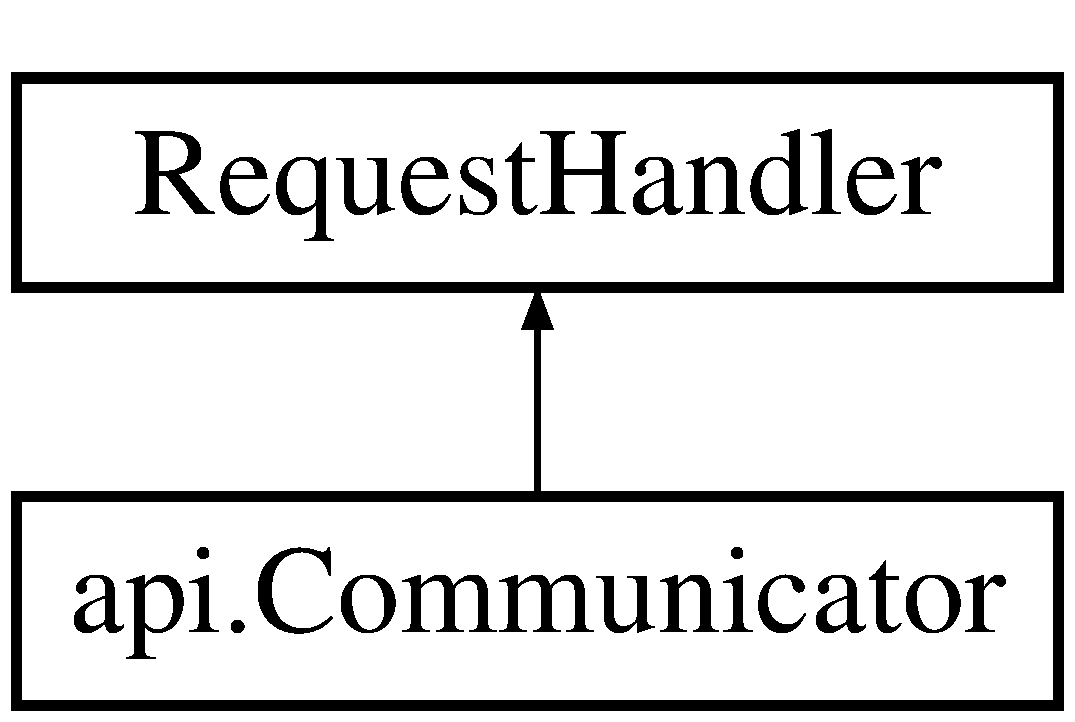
\includegraphics[height=2.000000cm]{classapi_1_1_communicator}
\end{center}
\end{figure}
\subsection*{Public Member Functions}
\begin{DoxyCompactItemize}
\item 
\hypertarget{classapi_1_1_communicator_a52ef801f9faaf4195e3824aba8ac1d65}{def {\bfseries initialize}}\label{classapi_1_1_communicator_a52ef801f9faaf4195e3824aba8ac1d65}

\item 
def \hyperlink{classapi_1_1_communicator_abc45b289619e0988116e80b35b7fabb9}{get}
\item 
def \hyperlink{classapi_1_1_communicator_acf9eee605fa05aafd4ef7b9caa7e3064}{post}
\item 
def \hyperlink{classapi_1_1_communicator_a7b1910fd8ee6416508032e9c533634da}{delete}
\item 
def \hyperlink{classapi_1_1_communicator_af5958bce2d64cec51a03c6c27b44122c}{put}
\end{DoxyCompactItemize}
\subsection*{Public Attributes}
\begin{DoxyCompactItemize}
\item 
\hypertarget{classapi_1_1_communicator_ad81c8f11473c4779f45fb7ca8993b5bd}{{\bfseries nest\-Id}}\label{classapi_1_1_communicator_ad81c8f11473c4779f45fb7ca8993b5bd}

\end{DoxyCompactItemize}


\subsection{Member Function Documentation}
\hypertarget{classapi_1_1_communicator_a7b1910fd8ee6416508032e9c533634da}{\index{api\-::\-Communicator@{api\-::\-Communicator}!delete@{delete}}
\index{delete@{delete}!api::Communicator@{api\-::\-Communicator}}
\subsubsection[{delete}]{\setlength{\rightskip}{0pt plus 5cm}def api.\-Communicator.\-delete (
\begin{DoxyParamCaption}
\item[{}]{self, }
\item[{}]{nest\-Id}
\end{DoxyParamCaption}
)}}\label{classapi_1_1_communicator_a7b1910fd8ee6416508032e9c533634da}
\begin{DoxyVerb}DELETE: ends the currently open communication session between members of a Nest.\end{DoxyVerb}
 \hypertarget{classapi_1_1_communicator_abc45b289619e0988116e80b35b7fabb9}{\index{api\-::\-Communicator@{api\-::\-Communicator}!get@{get}}
\index{get@{get}!api::Communicator@{api\-::\-Communicator}}
\subsubsection[{get}]{\setlength{\rightskip}{0pt plus 5cm}def api.\-Communicator.\-get (
\begin{DoxyParamCaption}
\item[{}]{self, }
\item[{}]{nest\-Id}
\end{DoxyParamCaption}
)}}\label{classapi_1_1_communicator_abc45b289619e0988116e80b35b7fabb9}
\begin{DoxyVerb}GET: gets the current communication session opened between members of a Nest, or null if uninitiated.\end{DoxyVerb}
 \hypertarget{classapi_1_1_communicator_acf9eee605fa05aafd4ef7b9caa7e3064}{\index{api\-::\-Communicator@{api\-::\-Communicator}!post@{post}}
\index{post@{post}!api::Communicator@{api\-::\-Communicator}}
\subsubsection[{post}]{\setlength{\rightskip}{0pt plus 5cm}def api.\-Communicator.\-post (
\begin{DoxyParamCaption}
\item[{}]{self, }
\item[{}]{nest\-Id}
\end{DoxyParamCaption}
)}}\label{classapi_1_1_communicator_acf9eee605fa05aafd4ef7b9caa7e3064}
\begin{DoxyVerb}POST: starts a new communication session between members of a Nest.\end{DoxyVerb}
 \hypertarget{classapi_1_1_communicator_af5958bce2d64cec51a03c6c27b44122c}{\index{api\-::\-Communicator@{api\-::\-Communicator}!put@{put}}
\index{put@{put}!api::Communicator@{api\-::\-Communicator}}
\subsubsection[{put}]{\setlength{\rightskip}{0pt plus 5cm}def api.\-Communicator.\-put (
\begin{DoxyParamCaption}
\item[{}]{self, }
\item[{}]{nest\-Id}
\end{DoxyParamCaption}
)}}\label{classapi_1_1_communicator_af5958bce2d64cec51a03c6c27b44122c}
\begin{DoxyVerb}PUT: updates the currently open communication session between members of a Nest.\end{DoxyVerb}
 

The documentation for this class was generated from the following file\-:\begin{DoxyCompactItemize}
\item 
api.\-py\end{DoxyCompactItemize}

\hypertarget{class_canary_assets_1_1_device_1_1_device}{\section{Canary\-Assets.\-Device.\-Device Class Reference}
\label{class_canary_assets_1_1_device_1_1_device}\index{Canary\-Assets.\-Device.\-Device@{Canary\-Assets.\-Device.\-Device}}
}
Inheritance diagram for Canary\-Assets.\-Device.\-Device\-:\begin{figure}[H]
\begin{center}
\leavevmode
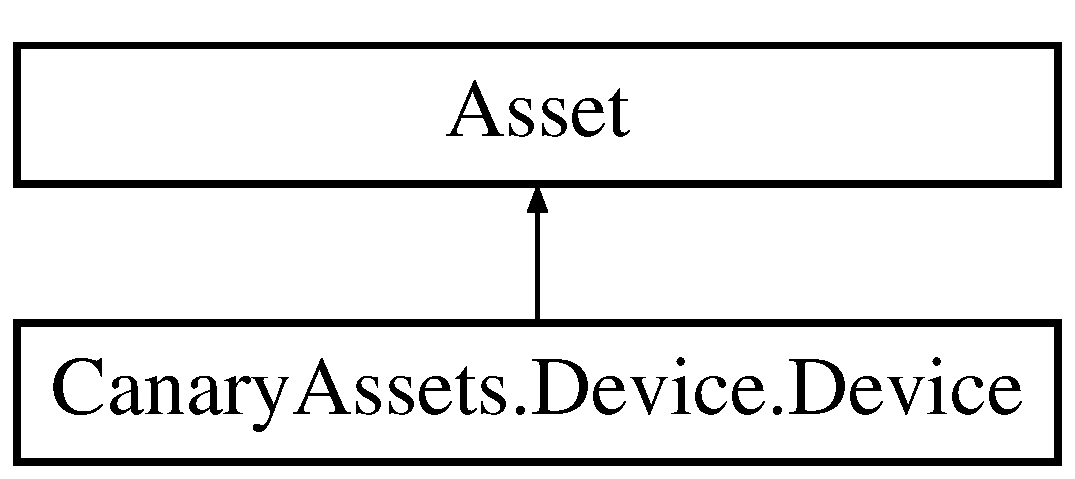
\includegraphics[height=2.000000cm]{class_canary_assets_1_1_device_1_1_device}
\end{center}
\end{figure}
\subsection*{Public Member Functions}
\begin{DoxyCompactItemize}
\item 
\hypertarget{class_canary_assets_1_1_device_1_1_device_ae1491c142e011fd608d2bf185a398d73}{def {\bfseries \-\_\-\-\_\-init\-\_\-\-\_\-}}\label{class_canary_assets_1_1_device_1_1_device_ae1491c142e011fd608d2bf185a398d73}

\item 
def \hyperlink{class_canary_assets_1_1_device_1_1_device_ad06a4aeb7c5e74c4714874cce699ce4c}{create}
\item 
def \hyperlink{class_canary_assets_1_1_device_1_1_device_aa923fdac7f6bf5cb504f857fde36d92f}{add\-To\-Nest}
\item 
def \hyperlink{class_canary_assets_1_1_device_1_1_device_a170ceac43e5fc92c64d75a022c165b2e}{remove\-From\-Nest}
\end{DoxyCompactItemize}
\subsection*{Public Attributes}
\begin{DoxyCompactItemize}
\item 
\hypertarget{class_canary_assets_1_1_device_1_1_device_a019c36f9397232cb1f7b9b81da49aad5}{{\bfseries status}}\label{class_canary_assets_1_1_device_1_1_device_a019c36f9397232cb1f7b9b81da49aad5}

\end{DoxyCompactItemize}


\subsection{Member Function Documentation}
\hypertarget{class_canary_assets_1_1_device_1_1_device_aa923fdac7f6bf5cb504f857fde36d92f}{\index{Canary\-Assets\-::\-Device\-::\-Device@{Canary\-Assets\-::\-Device\-::\-Device}!add\-To\-Nest@{add\-To\-Nest}}
\index{add\-To\-Nest@{add\-To\-Nest}!CanaryAssets::Device::Device@{Canary\-Assets\-::\-Device\-::\-Device}}
\subsubsection[{add\-To\-Nest}]{\setlength{\rightskip}{0pt plus 5cm}def Canary\-Assets.\-Device.\-Device.\-add\-To\-Nest (
\begin{DoxyParamCaption}
\item[{}]{self, }
\item[{}]{nest\-Id = {\ttfamily None}}
\end{DoxyParamCaption}
)}}\label{class_canary_assets_1_1_device_1_1_device_aa923fdac7f6bf5cb504f857fde36d92f}
\begin{DoxyVerb}Adds Device to a Nest\end{DoxyVerb}
 \hypertarget{class_canary_assets_1_1_device_1_1_device_ad06a4aeb7c5e74c4714874cce699ce4c}{\index{Canary\-Assets\-::\-Device\-::\-Device@{Canary\-Assets\-::\-Device\-::\-Device}!create@{create}}
\index{create@{create}!CanaryAssets::Device::Device@{Canary\-Assets\-::\-Device\-::\-Device}}
\subsubsection[{create}]{\setlength{\rightskip}{0pt plus 5cm}def Canary\-Assets.\-Device.\-Device.\-create (
\begin{DoxyParamCaption}
\item[{}]{self}
\end{DoxyParamCaption}
)}}\label{class_canary_assets_1_1_device_1_1_device_ad06a4aeb7c5e74c4714874cce699ce4c}
\begin{DoxyVerb}Creates a new Device, and sets its id.\end{DoxyVerb}
 \hypertarget{class_canary_assets_1_1_device_1_1_device_a170ceac43e5fc92c64d75a022c165b2e}{\index{Canary\-Assets\-::\-Device\-::\-Device@{Canary\-Assets\-::\-Device\-::\-Device}!remove\-From\-Nest@{remove\-From\-Nest}}
\index{remove\-From\-Nest@{remove\-From\-Nest}!CanaryAssets::Device::Device@{Canary\-Assets\-::\-Device\-::\-Device}}
\subsubsection[{remove\-From\-Nest}]{\setlength{\rightskip}{0pt plus 5cm}def Canary\-Assets.\-Device.\-Device.\-remove\-From\-Nest (
\begin{DoxyParamCaption}
\item[{}]{self, }
\item[{}]{nest\-Id = {\ttfamily None}}
\end{DoxyParamCaption}
)}}\label{class_canary_assets_1_1_device_1_1_device_a170ceac43e5fc92c64d75a022c165b2e}
\begin{DoxyVerb}Removes Device from a Nest\end{DoxyVerb}
 

The documentation for this class was generated from the following file\-:\begin{DoxyCompactItemize}
\item 
Canary\-Assets/Device.\-py\end{DoxyCompactItemize}

\hypertarget{classapi_1_1_device}{\section{api.\-Device Class Reference}
\label{classapi_1_1_device}\index{api.\-Device@{api.\-Device}}
}
Inheritance diagram for api.\-Device\-:\begin{figure}[H]
\begin{center}
\leavevmode
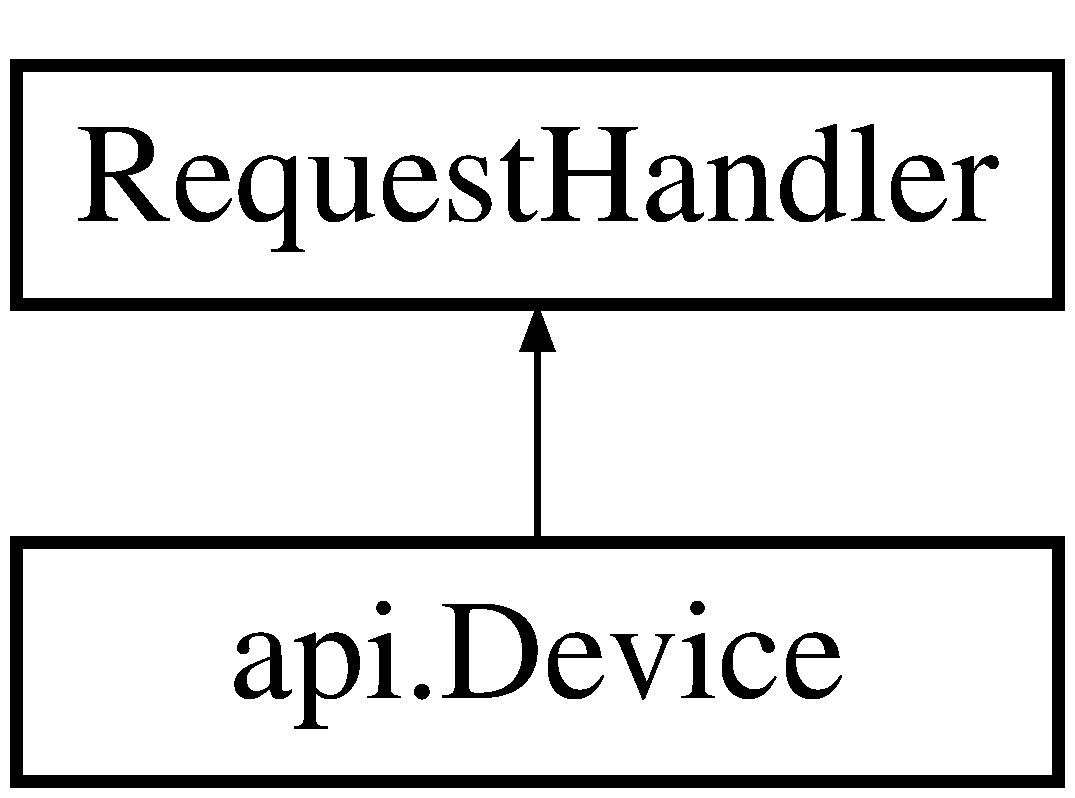
\includegraphics[height=2.000000cm]{classapi_1_1_device}
\end{center}
\end{figure}
\subsection*{Public Member Functions}
\begin{DoxyCompactItemize}
\item 
\hypertarget{classapi_1_1_device_abe43b29a0471c001944bb1634ead3165}{def {\bfseries initialize}}\label{classapi_1_1_device_abe43b29a0471c001944bb1634ead3165}

\item 
def \hyperlink{classapi_1_1_device_aab84744b823a1e3f44700c9ba50d5051}{get}
\item 
def \hyperlink{classapi_1_1_device_ae051140ce5b14440b74a6634c27ee4c0}{put}
\item 
def \hyperlink{classapi_1_1_device_aa1b4c05ad4a3331e80331754055c0ec9}{delete}
\end{DoxyCompactItemize}
\subsection*{Public Attributes}
\begin{DoxyCompactItemize}
\item 
\hypertarget{classapi_1_1_device_a0190a4c54d0998cd83368e9b99b9cfdf}{{\bfseries device\-Id}}\label{classapi_1_1_device_a0190a4c54d0998cd83368e9b99b9cfdf}

\end{DoxyCompactItemize}


\subsection{Member Function Documentation}
\hypertarget{classapi_1_1_device_aa1b4c05ad4a3331e80331754055c0ec9}{\index{api\-::\-Device@{api\-::\-Device}!delete@{delete}}
\index{delete@{delete}!api::Device@{api\-::\-Device}}
\subsubsection[{delete}]{\setlength{\rightskip}{0pt plus 5cm}def api.\-Device.\-delete (
\begin{DoxyParamCaption}
\item[{}]{self, }
\item[{}]{device\-Id}
\end{DoxyParamCaption}
)}}\label{classapi_1_1_device_aa1b4c05ad4a3331e80331754055c0ec9}
\begin{DoxyVerb}DELETE: deletes the Device.\end{DoxyVerb}
 \hypertarget{classapi_1_1_device_aab84744b823a1e3f44700c9ba50d5051}{\index{api\-::\-Device@{api\-::\-Device}!get@{get}}
\index{get@{get}!api::Device@{api\-::\-Device}}
\subsubsection[{get}]{\setlength{\rightskip}{0pt plus 5cm}def api.\-Device.\-get (
\begin{DoxyParamCaption}
\item[{}]{self, }
\item[{}]{device\-Id}
\end{DoxyParamCaption}
)}}\label{classapi_1_1_device_aab84744b823a1e3f44700c9ba50d5051}
\begin{DoxyVerb}GET: returns the Device matching specified id.\end{DoxyVerb}
 \hypertarget{classapi_1_1_device_ae051140ce5b14440b74a6634c27ee4c0}{\index{api\-::\-Device@{api\-::\-Device}!put@{put}}
\index{put@{put}!api::Device@{api\-::\-Device}}
\subsubsection[{put}]{\setlength{\rightskip}{0pt plus 5cm}def api.\-Device.\-put (
\begin{DoxyParamCaption}
\item[{}]{self, }
\item[{}]{device\-Id}
\end{DoxyParamCaption}
)}}\label{classapi_1_1_device_ae051140ce5b14440b74a6634c27ee4c0}
\begin{DoxyVerb}PUT: updates the Device's data.\end{DoxyVerb}
 

The documentation for this class was generated from the following file\-:\begin{DoxyCompactItemize}
\item 
api.\-py\end{DoxyCompactItemize}

\hypertarget{classapi_1_1_devices}{\section{api.\-Devices Class Reference}
\label{classapi_1_1_devices}\index{api.\-Devices@{api.\-Devices}}
}
Inheritance diagram for api.\-Devices\-:\begin{figure}[H]
\begin{center}
\leavevmode
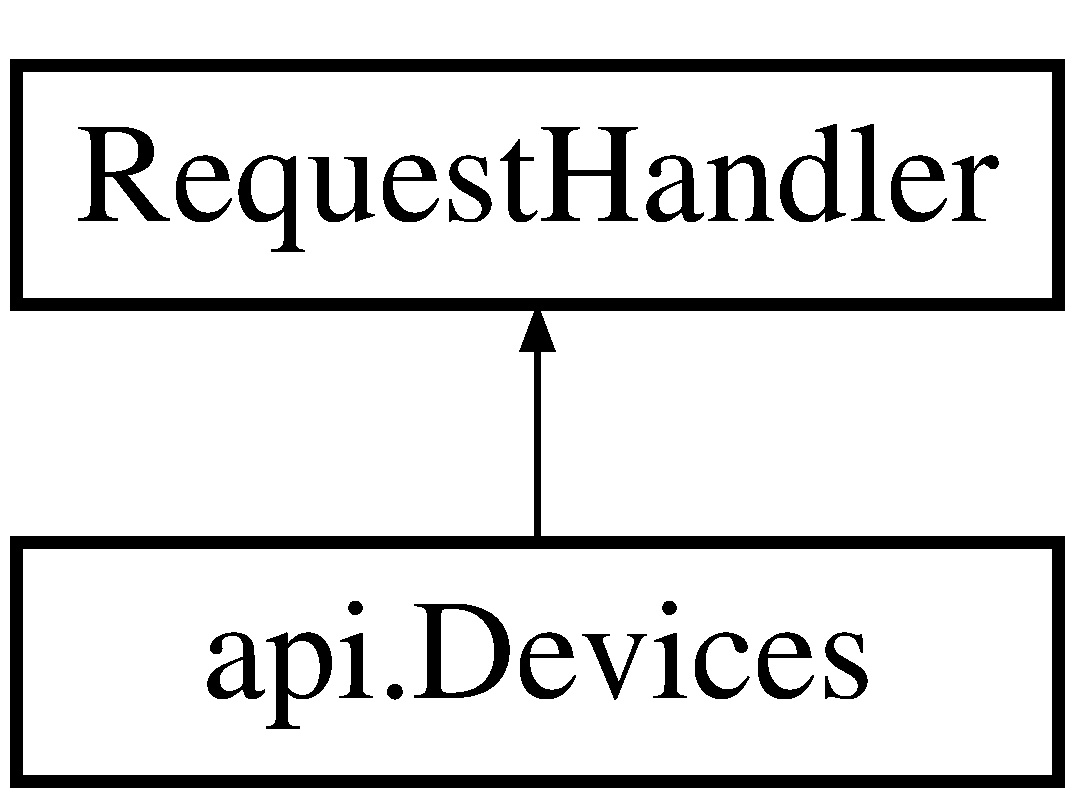
\includegraphics[height=2.000000cm]{classapi_1_1_devices}
\end{center}
\end{figure}
\subsection*{Public Member Functions}
\begin{DoxyCompactItemize}
\item 
def \hyperlink{classapi_1_1_devices_a695093fde641d0b21cecfca0c3c9d4c0}{get}
\item 
def \hyperlink{classapi_1_1_devices_accb6dbcf0fa656cfbab95553867ece1b}{post}
\end{DoxyCompactItemize}


\subsection{Member Function Documentation}
\hypertarget{classapi_1_1_devices_a695093fde641d0b21cecfca0c3c9d4c0}{\index{api\-::\-Devices@{api\-::\-Devices}!get@{get}}
\index{get@{get}!api::Devices@{api\-::\-Devices}}
\subsubsection[{get}]{\setlength{\rightskip}{0pt plus 5cm}def api.\-Devices.\-get (
\begin{DoxyParamCaption}
\item[{}]{self}
\end{DoxyParamCaption}
)}}\label{classapi_1_1_devices_a695093fde641d0b21cecfca0c3c9d4c0}
\begin{DoxyVerb}GET: returns the Devices registered.\end{DoxyVerb}
 \hypertarget{classapi_1_1_devices_accb6dbcf0fa656cfbab95553867ece1b}{\index{api\-::\-Devices@{api\-::\-Devices}!post@{post}}
\index{post@{post}!api::Devices@{api\-::\-Devices}}
\subsubsection[{post}]{\setlength{\rightskip}{0pt plus 5cm}def api.\-Devices.\-post (
\begin{DoxyParamCaption}
\item[{}]{self}
\end{DoxyParamCaption}
)}}\label{classapi_1_1_devices_accb6dbcf0fa656cfbab95553867ece1b}
\begin{DoxyVerb}POST: adds a new Device.

Post data must contain valid Device object.
\end{DoxyVerb}
 

The documentation for this class was generated from the following file\-:\begin{DoxyCompactItemize}
\item 
api.\-py\end{DoxyCompactItemize}

\hypertarget{classhailingfrequency_1_1_hailing_frequency}{\section{hailingfrequency.\-Hailing\-Frequency Class Reference}
\label{classhailingfrequency_1_1_hailing_frequency}\index{hailingfrequency.\-Hailing\-Frequency@{hailingfrequency.\-Hailing\-Frequency}}
}
Inheritance diagram for hailingfrequency.\-Hailing\-Frequency\-:\begin{figure}[H]
\begin{center}
\leavevmode
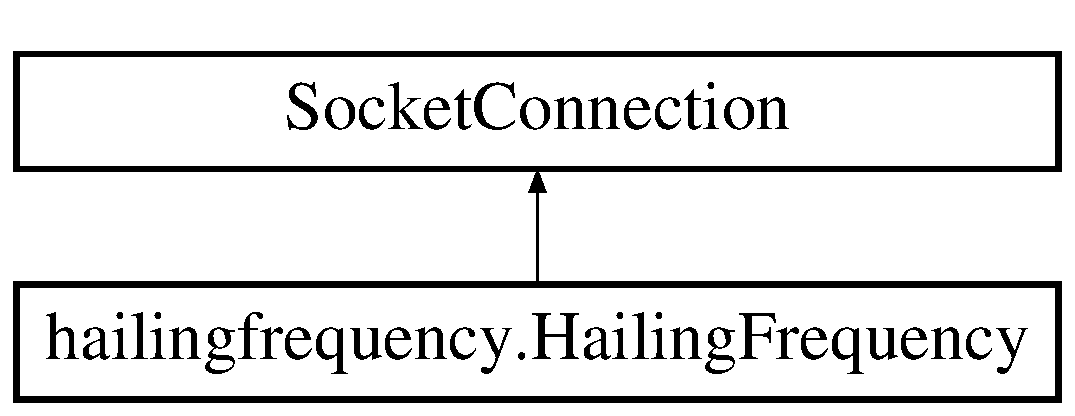
\includegraphics[height=2.000000cm]{classhailingfrequency_1_1_hailing_frequency}
\end{center}
\end{figure}
\subsection*{Public Member Functions}
\begin{DoxyCompactItemize}
\item 
\hypertarget{classhailingfrequency_1_1_hailing_frequency_a43ef95e6ea485f5d6f3237cffcffc2e8}{def {\bfseries on\-\_\-open}}\label{classhailingfrequency_1_1_hailing_frequency_a43ef95e6ea485f5d6f3237cffcffc2e8}

\item 
\hypertarget{classhailingfrequency_1_1_hailing_frequency_a6cd98bd788ac92a75717ea4eebc7ece5}{def {\bfseries on\-\_\-message}}\label{classhailingfrequency_1_1_hailing_frequency_a6cd98bd788ac92a75717ea4eebc7ece5}

\item 
\hypertarget{classhailingfrequency_1_1_hailing_frequency_a2b4502d47401f769da2d025af35df25e}{def {\bfseries on\-\_\-close}}\label{classhailingfrequency_1_1_hailing_frequency_a2b4502d47401f769da2d025af35df25e}

\end{DoxyCompactItemize}
\subsection*{Static Public Attributes}
\begin{DoxyCompactItemize}
\item 
\hypertarget{classhailingfrequency_1_1_hailing_frequency_a0e09ad983a40863402e49ed9e69e463d}{tuple {\bfseries participants} = set()}\label{classhailingfrequency_1_1_hailing_frequency_a0e09ad983a40863402e49ed9e69e463d}

\end{DoxyCompactItemize}


The documentation for this class was generated from the following file\-:\begin{DoxyCompactItemize}
\item 
hailingfrequency.\-py\end{DoxyCompactItemize}

\hypertarget{classhailingfrequency_1_1_hailing_frequency_handler}{\section{hailingfrequency.\-Hailing\-Frequency\-Handler Class Reference}
\label{classhailingfrequency_1_1_hailing_frequency_handler}\index{hailingfrequency.\-Hailing\-Frequency\-Handler@{hailingfrequency.\-Hailing\-Frequency\-Handler}}
}
Inheritance diagram for hailingfrequency.\-Hailing\-Frequency\-Handler\-:\begin{figure}[H]
\begin{center}
\leavevmode
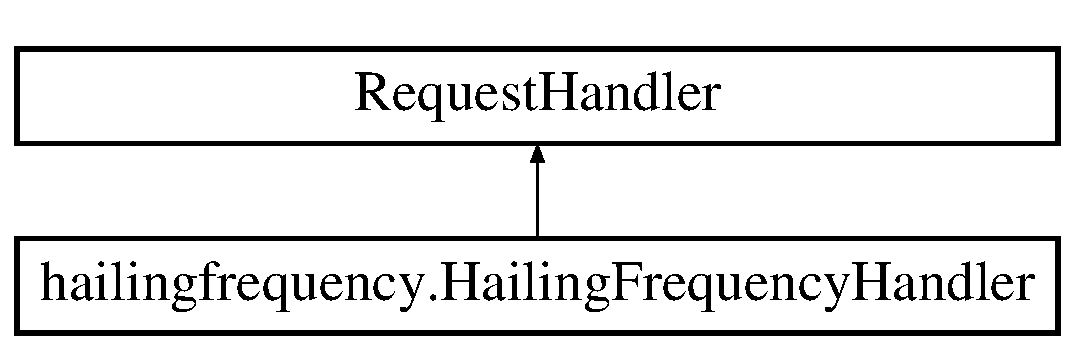
\includegraphics[height=2.000000cm]{classhailingfrequency_1_1_hailing_frequency_handler}
\end{center}
\end{figure}
\subsection*{Public Member Functions}
\begin{DoxyCompactItemize}
\item 
\hypertarget{classhailingfrequency_1_1_hailing_frequency_handler_a0bda90585d0261bea07e6db3077d6f79}{def {\bfseries get}}\label{classhailingfrequency_1_1_hailing_frequency_handler_a0bda90585d0261bea07e6db3077d6f79}

\end{DoxyCompactItemize}


The documentation for this class was generated from the following file\-:\begin{DoxyCompactItemize}
\item 
hailingfrequency.\-py\end{DoxyCompactItemize}

\hypertarget{class_canary_models_1_1_model_1_1_model}{\section{Canary\-Models.\-Model.\-Model Class Reference}
\label{class_canary_models_1_1_model_1_1_model}\index{Canary\-Models.\-Model.\-Model@{Canary\-Models.\-Model.\-Model}}
}
\subsection*{Public Member Functions}
\begin{DoxyCompactItemize}
\item 
\hypertarget{class_canary_models_1_1_model_1_1_model_a3125982406bc3fb9edd8695282c40170}{def {\bfseries \-\_\-\-\_\-init\-\_\-\-\_\-}}\label{class_canary_models_1_1_model_1_1_model_a3125982406bc3fb9edd8695282c40170}

\item 
def \hyperlink{class_canary_models_1_1_model_1_1_model_afd755af4b83ed6b3559c2ebb3272c3cf}{calculate\-Score}
\item 
def \hyperlink{class_canary_models_1_1_model_1_1_model_ad4ba832351ccfc18604c51a338a6848e}{emit}
\end{DoxyCompactItemize}


\subsection{Detailed Description}
\begin{DoxyVerb}The Model superclass encapsulates all data objects that record, calculate, and emit real-time metric data, such as temperature readings, co2, battery, etc.\end{DoxyVerb}
 

\subsection{Member Function Documentation}
\hypertarget{class_canary_models_1_1_model_1_1_model_afd755af4b83ed6b3559c2ebb3272c3cf}{\index{Canary\-Models\-::\-Model\-::\-Model@{Canary\-Models\-::\-Model\-::\-Model}!calculate\-Score@{calculate\-Score}}
\index{calculate\-Score@{calculate\-Score}!CanaryModels::Model::Model@{Canary\-Models\-::\-Model\-::\-Model}}
\subsubsection[{calculate\-Score}]{\setlength{\rightskip}{0pt plus 5cm}def Canary\-Models.\-Model.\-Model.\-calculate\-Score (
\begin{DoxyParamCaption}
\item[{}]{self}
\end{DoxyParamCaption}
)}}\label{class_canary_models_1_1_model_1_1_model_afd755af4b83ed6b3559c2ebb3272c3cf}
\begin{DoxyVerb}Calculates the floating point value of the given metric.  This method must be overridden by the subclass using it, as each metric has a unique way of being calculated.\end{DoxyVerb}
 \hypertarget{class_canary_models_1_1_model_1_1_model_ad4ba832351ccfc18604c51a338a6848e}{\index{Canary\-Models\-::\-Model\-::\-Model@{Canary\-Models\-::\-Model\-::\-Model}!emit@{emit}}
\index{emit@{emit}!CanaryModels::Model::Model@{Canary\-Models\-::\-Model\-::\-Model}}
\subsubsection[{emit}]{\setlength{\rightskip}{0pt plus 5cm}def Canary\-Models.\-Model.\-Model.\-emit (
\begin{DoxyParamCaption}
\item[{}]{self}
\end{DoxyParamCaption}
)}}\label{class_canary_models_1_1_model_1_1_model_ad4ba832351ccfc18604c51a338a6848e}
\begin{DoxyVerb}Returns a json-encoded representation of this object.\end{DoxyVerb}
 

The documentation for this class was generated from the following file\-:\begin{DoxyCompactItemize}
\item 
Canary\-Models/Model.\-py\end{DoxyCompactItemize}

\hypertarget{class_canary_models_1_1_nearby_hazard_1_1_nearby_hazard}{\section{Canary\-Models.\-Nearby\-Hazard.\-Nearby\-Hazard Class Reference}
\label{class_canary_models_1_1_nearby_hazard_1_1_nearby_hazard}\index{Canary\-Models.\-Nearby\-Hazard.\-Nearby\-Hazard@{Canary\-Models.\-Nearby\-Hazard.\-Nearby\-Hazard}}
}
Inheritance diagram for Canary\-Models.\-Nearby\-Hazard.\-Nearby\-Hazard\-:\begin{figure}[H]
\begin{center}
\leavevmode
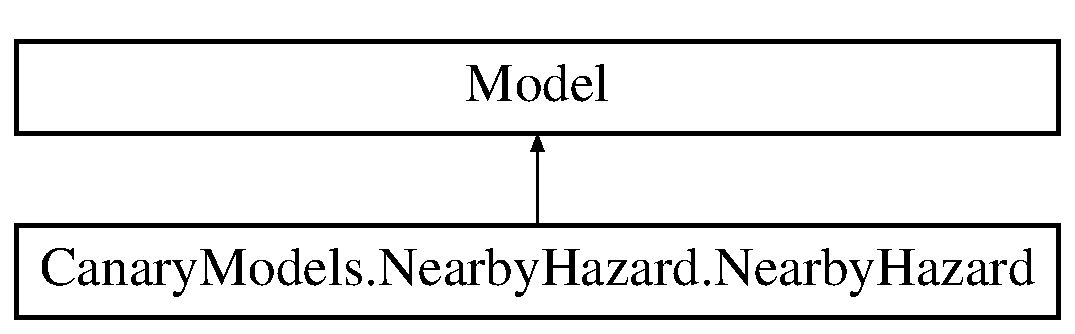
\includegraphics[height=2.000000cm]{class_canary_models_1_1_nearby_hazard_1_1_nearby_hazard}
\end{center}
\end{figure}
\subsection*{Public Member Functions}
\begin{DoxyCompactItemize}
\item 
\hypertarget{class_canary_models_1_1_nearby_hazard_1_1_nearby_hazard_ac9b77d72f77a5c5945e2064f21aaf334}{def {\bfseries \-\_\-\-\_\-init\-\_\-\-\_\-}}\label{class_canary_models_1_1_nearby_hazard_1_1_nearby_hazard_ac9b77d72f77a5c5945e2064f21aaf334}

\end{DoxyCompactItemize}


The documentation for this class was generated from the following file\-:\begin{DoxyCompactItemize}
\item 
Canary\-Models/Nearby\-Hazard.\-py\end{DoxyCompactItemize}

\hypertarget{classapi_1_1_nest}{\section{api.\-Nest Class Reference}
\label{classapi_1_1_nest}\index{api.\-Nest@{api.\-Nest}}
}
Inheritance diagram for api.\-Nest\-:\begin{figure}[H]
\begin{center}
\leavevmode
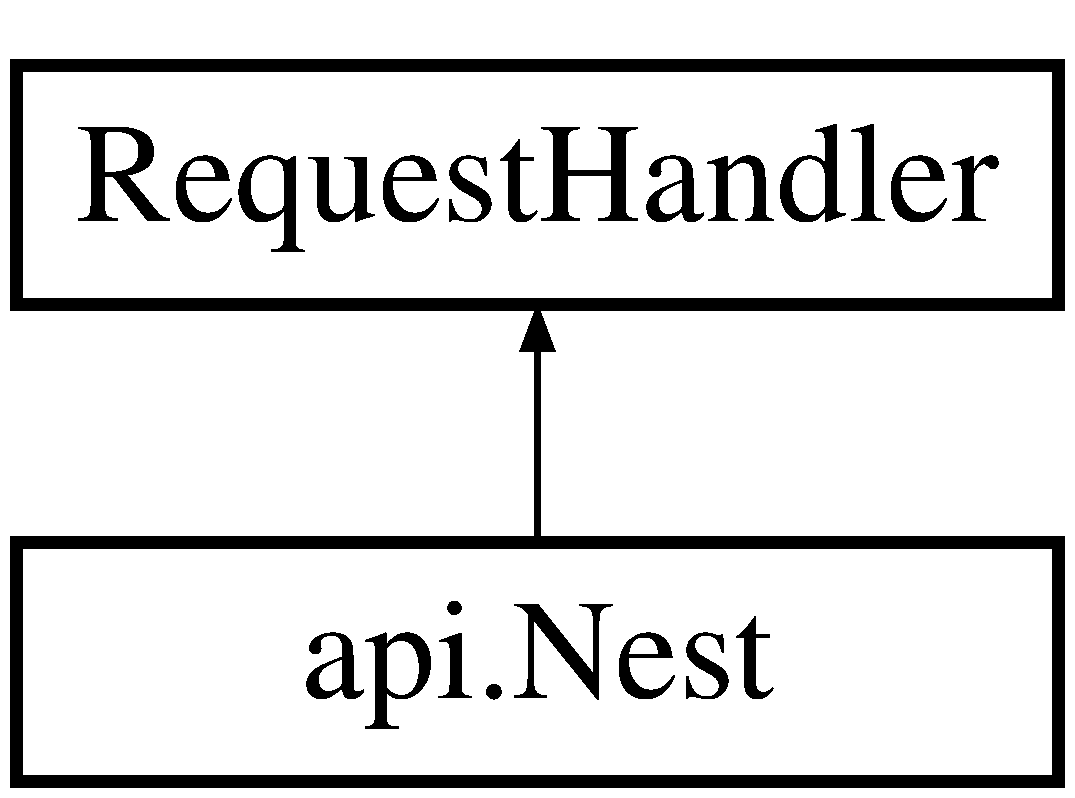
\includegraphics[height=2.000000cm]{classapi_1_1_nest}
\end{center}
\end{figure}
\subsection*{Public Member Functions}
\begin{DoxyCompactItemize}
\item 
\hypertarget{classapi_1_1_nest_ac63c05297a0c2a9ef7c4d78649bd6882}{def {\bfseries initialize}}\label{classapi_1_1_nest_ac63c05297a0c2a9ef7c4d78649bd6882}

\item 
def \hyperlink{classapi_1_1_nest_abc52411100635182cbd712b9f3014ea8}{get}
\item 
def \hyperlink{classapi_1_1_nest_a1b722ddb518afce74b5a59be42e7af09}{put}
\item 
def \hyperlink{classapi_1_1_nest_a224057785cc58de52b2fb5ba9edbb044}{delete}
\end{DoxyCompactItemize}
\subsection*{Public Attributes}
\begin{DoxyCompactItemize}
\item 
\hypertarget{classapi_1_1_nest_a4aae8cb29281cfd74c4c975fe309d612}{{\bfseries nest\-Id}}\label{classapi_1_1_nest_a4aae8cb29281cfd74c4c975fe309d612}

\end{DoxyCompactItemize}


\subsection{Member Function Documentation}
\hypertarget{classapi_1_1_nest_a224057785cc58de52b2fb5ba9edbb044}{\index{api\-::\-Nest@{api\-::\-Nest}!delete@{delete}}
\index{delete@{delete}!api::Nest@{api\-::\-Nest}}
\subsubsection[{delete}]{\setlength{\rightskip}{0pt plus 5cm}def api.\-Nest.\-delete (
\begin{DoxyParamCaption}
\item[{}]{self, }
\item[{}]{nest\-Id}
\end{DoxyParamCaption}
)}}\label{classapi_1_1_nest_a224057785cc58de52b2fb5ba9edbb044}
\begin{DoxyVerb}DELETE: deletes the Nest.\end{DoxyVerb}
 \hypertarget{classapi_1_1_nest_abc52411100635182cbd712b9f3014ea8}{\index{api\-::\-Nest@{api\-::\-Nest}!get@{get}}
\index{get@{get}!api::Nest@{api\-::\-Nest}}
\subsubsection[{get}]{\setlength{\rightskip}{0pt plus 5cm}def api.\-Nest.\-get (
\begin{DoxyParamCaption}
\item[{}]{self, }
\item[{}]{nest\-Id}
\end{DoxyParamCaption}
)}}\label{classapi_1_1_nest_abc52411100635182cbd712b9f3014ea8}
\begin{DoxyVerb}GET: returns the Nest matching specified id.\end{DoxyVerb}
 \hypertarget{classapi_1_1_nest_a1b722ddb518afce74b5a59be42e7af09}{\index{api\-::\-Nest@{api\-::\-Nest}!put@{put}}
\index{put@{put}!api::Nest@{api\-::\-Nest}}
\subsubsection[{put}]{\setlength{\rightskip}{0pt plus 5cm}def api.\-Nest.\-put (
\begin{DoxyParamCaption}
\item[{}]{self, }
\item[{}]{user\-Id}
\end{DoxyParamCaption}
)}}\label{classapi_1_1_nest_a1b722ddb518afce74b5a59be42e7af09}
\begin{DoxyVerb}PUT: updates the Nest's data.\end{DoxyVerb}
 

The documentation for this class was generated from the following file\-:\begin{DoxyCompactItemize}
\item 
api.\-py\end{DoxyCompactItemize}

\hypertarget{class_canary_assets_1_1_nest_1_1_nest}{\section{Canary\-Assets.\-Nest.\-Nest Class Reference}
\label{class_canary_assets_1_1_nest_1_1_nest}\index{Canary\-Assets.\-Nest.\-Nest@{Canary\-Assets.\-Nest.\-Nest}}
}
Inheritance diagram for Canary\-Assets.\-Nest.\-Nest\-:\begin{figure}[H]
\begin{center}
\leavevmode
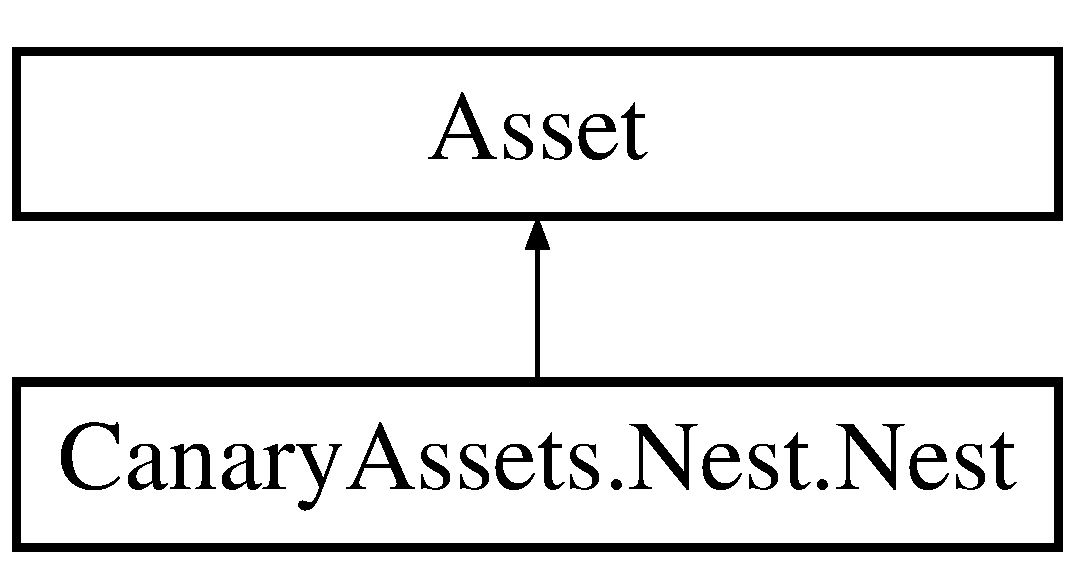
\includegraphics[height=2.000000cm]{class_canary_assets_1_1_nest_1_1_nest}
\end{center}
\end{figure}
\subsection*{Public Member Functions}
\begin{DoxyCompactItemize}
\item 
\hypertarget{class_canary_assets_1_1_nest_1_1_nest_a699269ce903225dca30cd976e4023e70}{def {\bfseries \-\_\-\-\_\-init\-\_\-\-\_\-}}\label{class_canary_assets_1_1_nest_1_1_nest_a699269ce903225dca30cd976e4023e70}

\item 
def \hyperlink{class_canary_assets_1_1_nest_1_1_nest_a557e617357bf28fcd96d31d980deeff9}{create}
\end{DoxyCompactItemize}
\subsection*{Public Attributes}
\begin{DoxyCompactItemize}
\item 
\hypertarget{class_canary_assets_1_1_nest_1_1_nest_aaf67343a84818206762d2578056b1f2a}{{\bfseries members}}\label{class_canary_assets_1_1_nest_1_1_nest_aaf67343a84818206762d2578056b1f2a}

\item 
\hypertarget{class_canary_assets_1_1_nest_1_1_nest_a9b1ae23c66abc485fb9f9d1402a0f5e2}{{\bfseries devices}}\label{class_canary_assets_1_1_nest_1_1_nest_a9b1ae23c66abc485fb9f9d1402a0f5e2}

\item 
\hypertarget{class_canary_assets_1_1_nest_1_1_nest_a03a0f34c05b34caa402609415dd7e12b}{{\bfseries quality}}\label{class_canary_assets_1_1_nest_1_1_nest_a03a0f34c05b34caa402609415dd7e12b}

\end{DoxyCompactItemize}


\subsection{Member Function Documentation}
\hypertarget{class_canary_assets_1_1_nest_1_1_nest_a557e617357bf28fcd96d31d980deeff9}{\index{Canary\-Assets\-::\-Nest\-::\-Nest@{Canary\-Assets\-::\-Nest\-::\-Nest}!create@{create}}
\index{create@{create}!CanaryAssets::Nest::Nest@{Canary\-Assets\-::\-Nest\-::\-Nest}}
\subsubsection[{create}]{\setlength{\rightskip}{0pt plus 5cm}def Canary\-Assets.\-Nest.\-Nest.\-create (
\begin{DoxyParamCaption}
\item[{}]{self}
\end{DoxyParamCaption}
)}}\label{class_canary_assets_1_1_nest_1_1_nest_a557e617357bf28fcd96d31d980deeff9}
\begin{DoxyVerb}Creates a new Nest, and sets its id.\end{DoxyVerb}
 

The documentation for this class was generated from the following file\-:\begin{DoxyCompactItemize}
\item 
Canary\-Assets/Nest.\-py\end{DoxyCompactItemize}

\hypertarget{classapi_1_1_nests}{\section{api.\-Nests Class Reference}
\label{classapi_1_1_nests}\index{api.\-Nests@{api.\-Nests}}
}
Inheritance diagram for api.\-Nests\-:\begin{figure}[H]
\begin{center}
\leavevmode
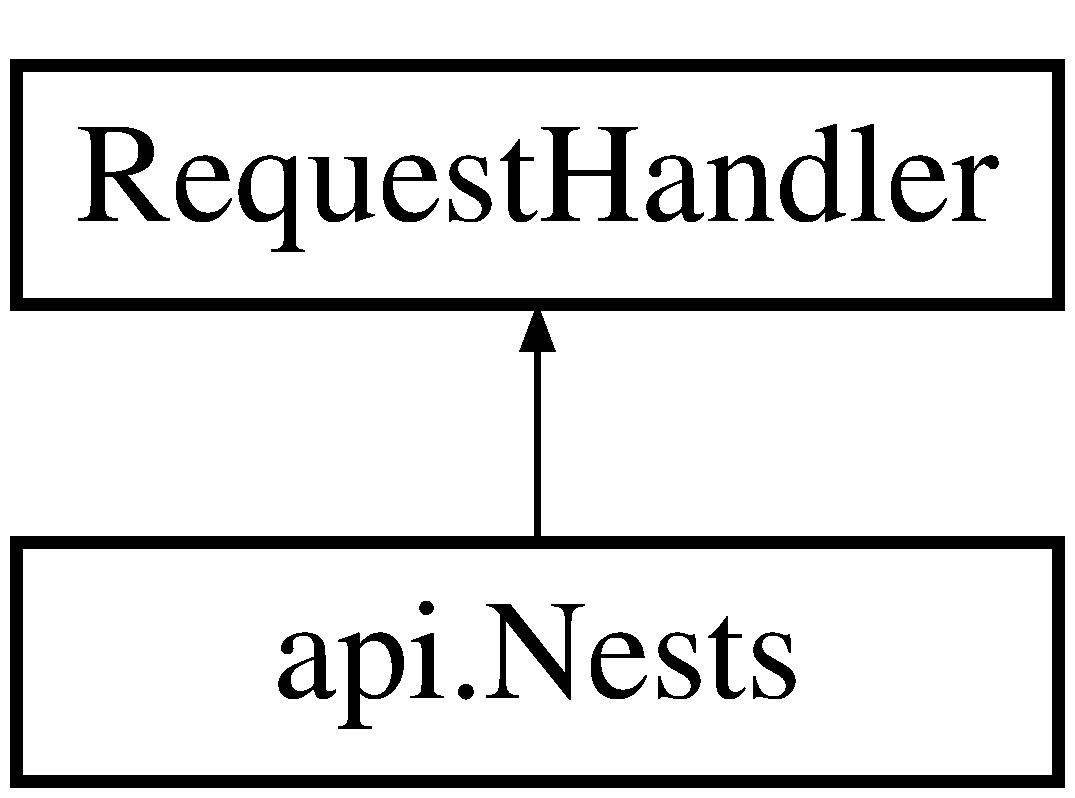
\includegraphics[height=2.000000cm]{classapi_1_1_nests}
\end{center}
\end{figure}
\subsection*{Public Member Functions}
\begin{DoxyCompactItemize}
\item 
def \hyperlink{classapi_1_1_nests_aee226cdcaacc8be98e80f1b27626f9ec}{get}
\item 
def \hyperlink{classapi_1_1_nests_aa0894a39e2ff51986c333fd19ef2cd34}{post}
\end{DoxyCompactItemize}


\subsection{Member Function Documentation}
\hypertarget{classapi_1_1_nests_aee226cdcaacc8be98e80f1b27626f9ec}{\index{api\-::\-Nests@{api\-::\-Nests}!get@{get}}
\index{get@{get}!api::Nests@{api\-::\-Nests}}
\subsubsection[{get}]{\setlength{\rightskip}{0pt plus 5cm}def api.\-Nests.\-get (
\begin{DoxyParamCaption}
\item[{}]{self}
\end{DoxyParamCaption}
)}}\label{classapi_1_1_nests_aee226cdcaacc8be98e80f1b27626f9ec}
\begin{DoxyVerb}GET: returns the Nests registered.\end{DoxyVerb}
 \hypertarget{classapi_1_1_nests_aa0894a39e2ff51986c333fd19ef2cd34}{\index{api\-::\-Nests@{api\-::\-Nests}!post@{post}}
\index{post@{post}!api::Nests@{api\-::\-Nests}}
\subsubsection[{post}]{\setlength{\rightskip}{0pt plus 5cm}def api.\-Nests.\-post (
\begin{DoxyParamCaption}
\item[{}]{self}
\end{DoxyParamCaption}
)}}\label{classapi_1_1_nests_aa0894a39e2ff51986c333fd19ef2cd34}
\begin{DoxyVerb}POST: adds a new Nest.

Post data must contain valid Nest object.
\end{DoxyVerb}
 

The documentation for this class was generated from the following file\-:\begin{DoxyCompactItemize}
\item 
api.\-py\end{DoxyCompactItemize}

\hypertarget{class_canary_models_1_1_n_o2_1_1_n_o2}{\section{Canary\-Models.\-N\-O2.\-N\-O2 Class Reference}
\label{class_canary_models_1_1_n_o2_1_1_n_o2}\index{Canary\-Models.\-N\-O2.\-N\-O2@{Canary\-Models.\-N\-O2.\-N\-O2}}
}
Inheritance diagram for Canary\-Models.\-N\-O2.\-N\-O2\-:\begin{figure}[H]
\begin{center}
\leavevmode
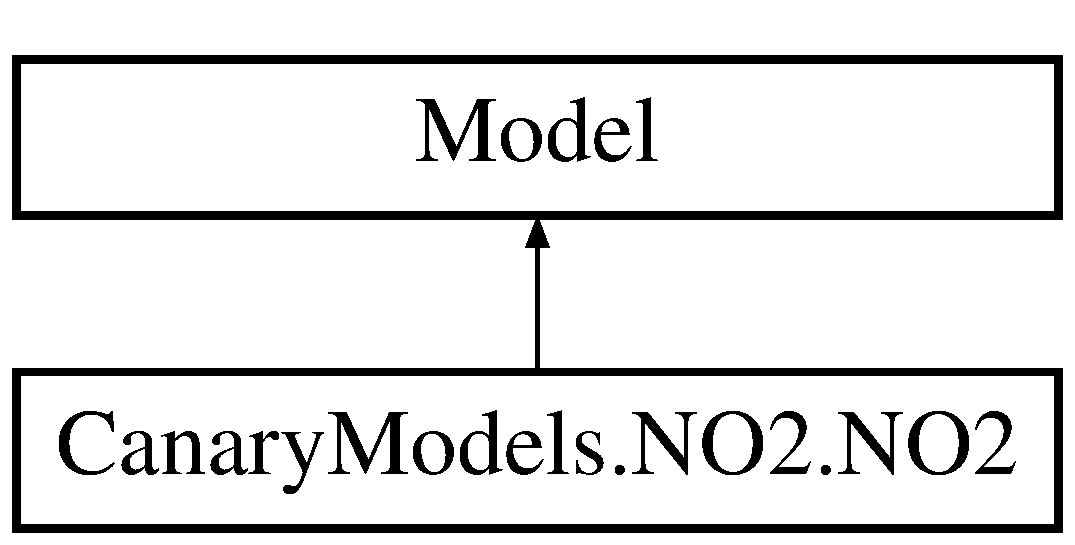
\includegraphics[height=2.000000cm]{class_canary_models_1_1_n_o2_1_1_n_o2}
\end{center}
\end{figure}
\subsection*{Public Member Functions}
\begin{DoxyCompactItemize}
\item 
\hypertarget{class_canary_models_1_1_n_o2_1_1_n_o2_ab72bcacce114176601574215f6143090}{def {\bfseries \-\_\-\-\_\-init\-\_\-\-\_\-}}\label{class_canary_models_1_1_n_o2_1_1_n_o2_ab72bcacce114176601574215f6143090}

\end{DoxyCompactItemize}


The documentation for this class was generated from the following file\-:\begin{DoxyCompactItemize}
\item 
Canary\-Models/N\-O2.\-py\end{DoxyCompactItemize}

\hypertarget{class_canary_models_1_1_outdoor_quality_1_1_outdoor_quality}{\section{Canary\-Models.\-Outdoor\-Quality.\-Outdoor\-Quality Class Reference}
\label{class_canary_models_1_1_outdoor_quality_1_1_outdoor_quality}\index{Canary\-Models.\-Outdoor\-Quality.\-Outdoor\-Quality@{Canary\-Models.\-Outdoor\-Quality.\-Outdoor\-Quality}}
}
Inheritance diagram for Canary\-Models.\-Outdoor\-Quality.\-Outdoor\-Quality\-:\begin{figure}[H]
\begin{center}
\leavevmode
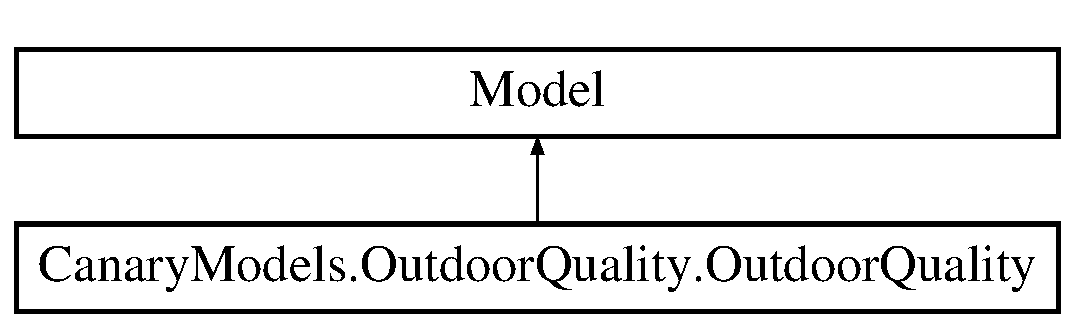
\includegraphics[height=2.000000cm]{class_canary_models_1_1_outdoor_quality_1_1_outdoor_quality}
\end{center}
\end{figure}
\subsection*{Public Member Functions}
\begin{DoxyCompactItemize}
\item 
\hypertarget{class_canary_models_1_1_outdoor_quality_1_1_outdoor_quality_a5257e4739c153fafc7d52201ebd85596}{def {\bfseries \-\_\-\-\_\-init\-\_\-\-\_\-}}\label{class_canary_models_1_1_outdoor_quality_1_1_outdoor_quality_a5257e4739c153fafc7d52201ebd85596}

\end{DoxyCompactItemize}


The documentation for this class was generated from the following file\-:\begin{DoxyCompactItemize}
\item 
Canary\-Models/Outdoor\-Quality.\-py\end{DoxyCompactItemize}

\hypertarget{classapi_1_1_ping}{\section{api.\-Ping Class Reference}
\label{classapi_1_1_ping}\index{api.\-Ping@{api.\-Ping}}
}
Inheritance diagram for api.\-Ping\-:\begin{figure}[H]
\begin{center}
\leavevmode
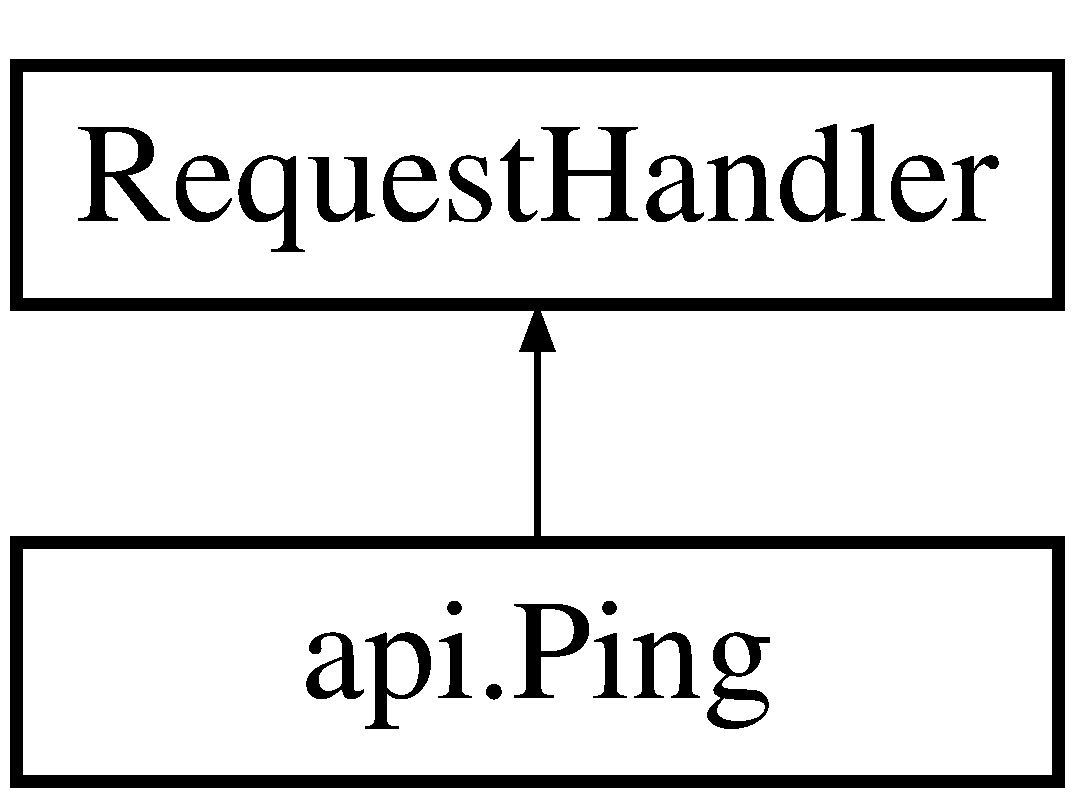
\includegraphics[height=2.000000cm]{classapi_1_1_ping}
\end{center}
\end{figure}
\subsection*{Public Member Functions}
\begin{DoxyCompactItemize}
\item 
\hypertarget{classapi_1_1_ping_a45732451f2e292e44dd204127920255d}{def {\bfseries initialize}}\label{classapi_1_1_ping_a45732451f2e292e44dd204127920255d}

\item 
def \hyperlink{classapi_1_1_ping_a6082e3e7608059cd50e92b116eaee580}{post}
\end{DoxyCompactItemize}
\subsection*{Public Attributes}
\begin{DoxyCompactItemize}
\item 
\hypertarget{classapi_1_1_ping_affa752457ec1a022bffd77fb58afc2b3}{{\bfseries entity\-Id}}\label{classapi_1_1_ping_affa752457ec1a022bffd77fb58afc2b3}

\item 
\hypertarget{classapi_1_1_ping_ae4e0ce63a966a74226524f07385b2cbe}{{\bfseries action}}\label{classapi_1_1_ping_ae4e0ce63a966a74226524f07385b2cbe}

\end{DoxyCompactItemize}


\subsection{Member Function Documentation}
\hypertarget{classapi_1_1_ping_a6082e3e7608059cd50e92b116eaee580}{\index{api\-::\-Ping@{api\-::\-Ping}!post@{post}}
\index{post@{post}!api::Ping@{api\-::\-Ping}}
\subsubsection[{post}]{\setlength{\rightskip}{0pt plus 5cm}def api.\-Ping.\-post (
\begin{DoxyParamCaption}
\item[{}]{self, }
\item[{}]{entity\-Id, }
\item[{}]{action\-Id}
\end{DoxyParamCaption}
)}}\label{classapi_1_1_ping_a6082e3e7608059cd50e92b116eaee580}
\begin{DoxyVerb}POST: sends a ping (event notification) to the specified entity, with action specified by the Action argument\end{DoxyVerb}
 

The documentation for this class was generated from the following file\-:\begin{DoxyCompactItemize}
\item 
api.\-py\end{DoxyCompactItemize}

\hypertarget{class_canary_models_1_1_p_m10_1_1_p_m10}{\section{Canary\-Models.\-P\-M10.\-P\-M10 Class Reference}
\label{class_canary_models_1_1_p_m10_1_1_p_m10}\index{Canary\-Models.\-P\-M10.\-P\-M10@{Canary\-Models.\-P\-M10.\-P\-M10}}
}
Inheritance diagram for Canary\-Models.\-P\-M10.\-P\-M10\-:\begin{figure}[H]
\begin{center}
\leavevmode
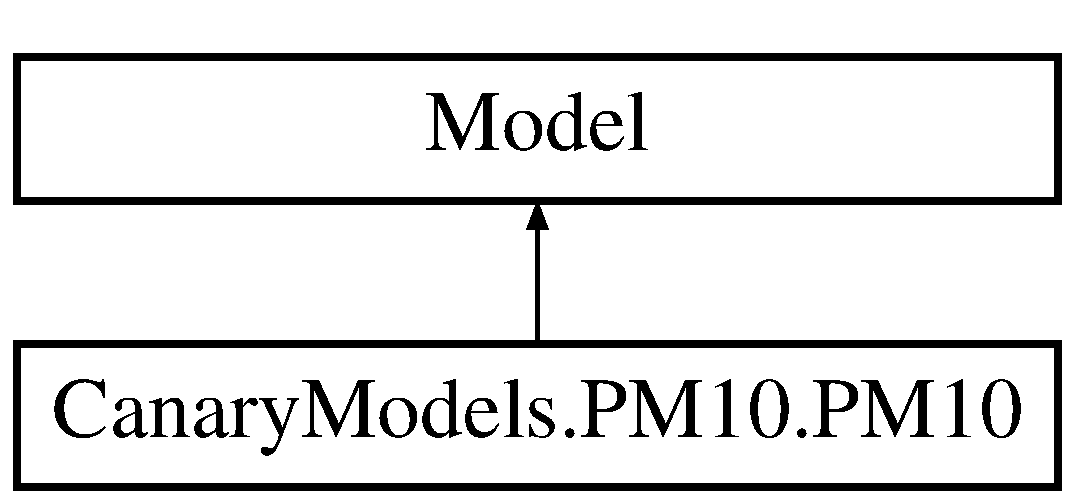
\includegraphics[height=2.000000cm]{class_canary_models_1_1_p_m10_1_1_p_m10}
\end{center}
\end{figure}
\subsection*{Public Member Functions}
\begin{DoxyCompactItemize}
\item 
\hypertarget{class_canary_models_1_1_p_m10_1_1_p_m10_a97395a9f40ca5ba05911ee8672a2c9aa}{def {\bfseries \-\_\-\-\_\-init\-\_\-\-\_\-}}\label{class_canary_models_1_1_p_m10_1_1_p_m10_a97395a9f40ca5ba05911ee8672a2c9aa}

\end{DoxyCompactItemize}


The documentation for this class was generated from the following file\-:\begin{DoxyCompactItemize}
\item 
Canary\-Models/P\-M10.\-py\end{DoxyCompactItemize}

\hypertarget{class_canary_models_1_1_p_m2__5_1_1_p_m2__5}{\section{Canary\-Models.\-P\-M2\-\_\-5.\-P\-M2\-\_\-5 Class Reference}
\label{class_canary_models_1_1_p_m2__5_1_1_p_m2__5}\index{Canary\-Models.\-P\-M2\-\_\-5.\-P\-M2\-\_\-5@{Canary\-Models.\-P\-M2\-\_\-5.\-P\-M2\-\_\-5}}
}
Inheritance diagram for Canary\-Models.\-P\-M2\-\_\-5.\-P\-M2\-\_\-5\-:\begin{figure}[H]
\begin{center}
\leavevmode
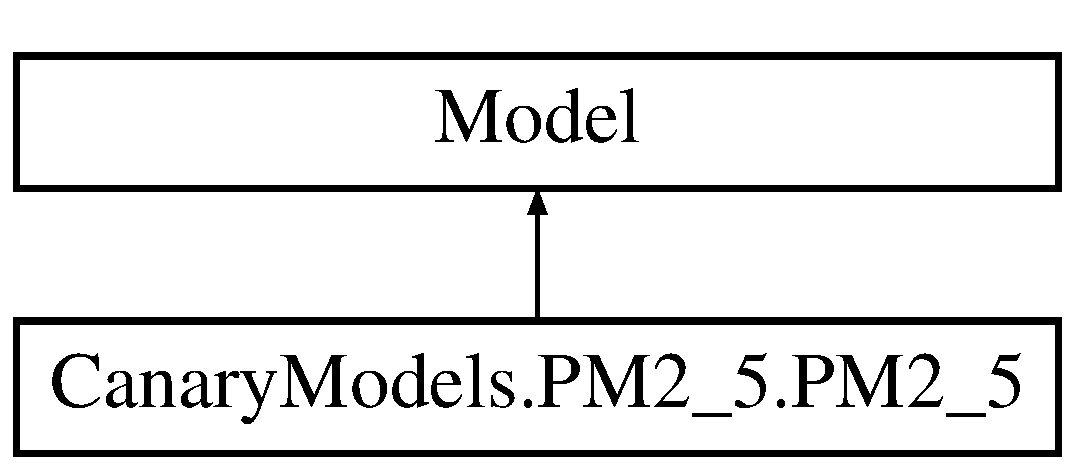
\includegraphics[height=2.000000cm]{class_canary_models_1_1_p_m2__5_1_1_p_m2__5}
\end{center}
\end{figure}
\subsection*{Public Member Functions}
\begin{DoxyCompactItemize}
\item 
\hypertarget{class_canary_models_1_1_p_m2__5_1_1_p_m2__5_a239dde2338017c639314d8f499b25149}{def {\bfseries \-\_\-\-\_\-init\-\_\-\-\_\-}}\label{class_canary_models_1_1_p_m2__5_1_1_p_m2__5_a239dde2338017c639314d8f499b25149}

\end{DoxyCompactItemize}


The documentation for this class was generated from the following file\-:\begin{DoxyCompactItemize}
\item 
Canary\-Models/P\-M2\-\_\-5.\-py\end{DoxyCompactItemize}

\hypertarget{classhailingfrequency_1_1_router}{\section{hailingfrequency.\-Router Class Reference}
\label{classhailingfrequency_1_1_router}\index{hailingfrequency.\-Router@{hailingfrequency.\-Router}}
}
Inheritance diagram for hailingfrequency.\-Router\-:\begin{figure}[H]
\begin{center}
\leavevmode
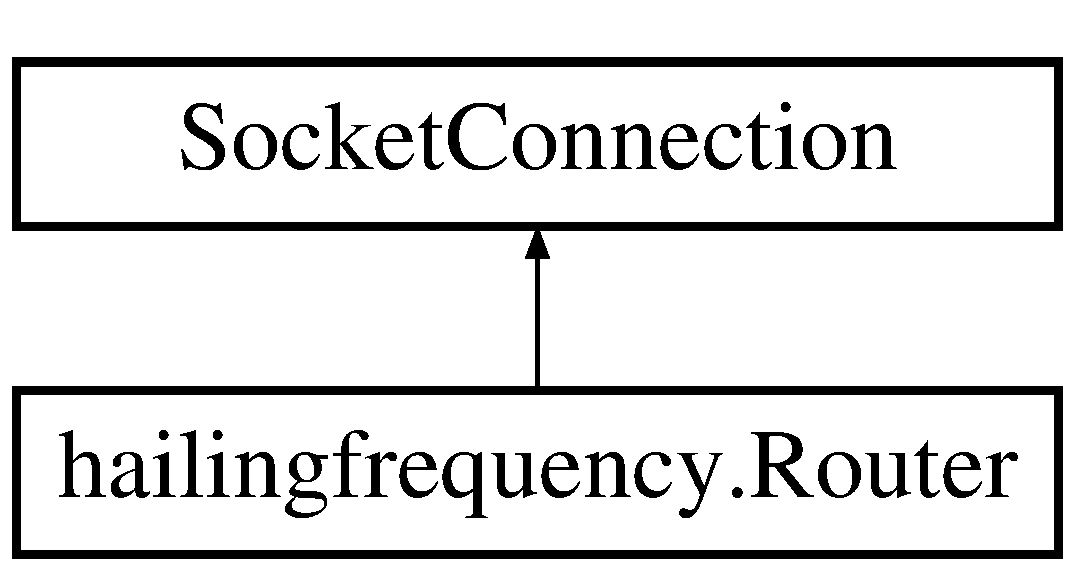
\includegraphics[height=2.000000cm]{classhailingfrequency_1_1_router}
\end{center}
\end{figure}
\subsection*{Static Public Attributes}
\begin{DoxyCompactItemize}
\item 
\hypertarget{classhailingfrequency_1_1_router_abd092ba4b038043ee08bc33112758c7a}{list {\bfseries ep} = \mbox{[}'/herpie','/derpie','/derpderp'\mbox{]}}\label{classhailingfrequency_1_1_router_abd092ba4b038043ee08bc33112758c7a}

\end{DoxyCompactItemize}


The documentation for this class was generated from the following file\-:\begin{DoxyCompactItemize}
\item 
hailingfrequency.\-py\end{DoxyCompactItemize}

\hypertarget{class_canary_models_1_1_smoke_1_1_smoke}{\section{Canary\-Models.\-Smoke.\-Smoke Class Reference}
\label{class_canary_models_1_1_smoke_1_1_smoke}\index{Canary\-Models.\-Smoke.\-Smoke@{Canary\-Models.\-Smoke.\-Smoke}}
}
Inheritance diagram for Canary\-Models.\-Smoke.\-Smoke\-:\begin{figure}[H]
\begin{center}
\leavevmode
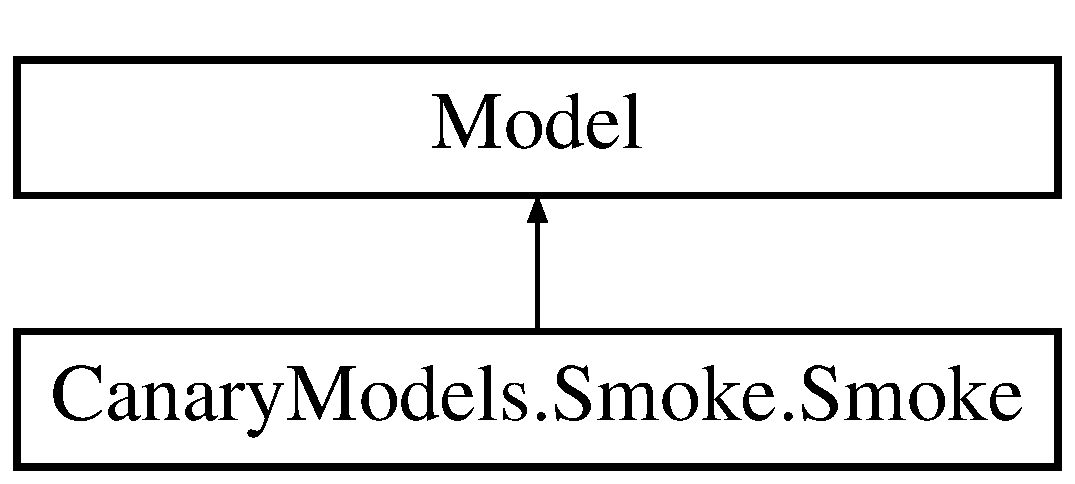
\includegraphics[height=2.000000cm]{class_canary_models_1_1_smoke_1_1_smoke}
\end{center}
\end{figure}
\subsection*{Public Member Functions}
\begin{DoxyCompactItemize}
\item 
\hypertarget{class_canary_models_1_1_smoke_1_1_smoke_a766f94eb787d6bb43280c98131fa127e}{def {\bfseries \-\_\-\-\_\-init\-\_\-\-\_\-}}\label{class_canary_models_1_1_smoke_1_1_smoke_a766f94eb787d6bb43280c98131fa127e}

\end{DoxyCompactItemize}


The documentation for this class was generated from the following file\-:\begin{DoxyCompactItemize}
\item 
Canary\-Models/Smoke.\-py\end{DoxyCompactItemize}

\hypertarget{classhailingfrequency_1_1_socket_i_o_handler}{\section{hailingfrequency.\-Socket\-I\-O\-Handler Class Reference}
\label{classhailingfrequency_1_1_socket_i_o_handler}\index{hailingfrequency.\-Socket\-I\-O\-Handler@{hailingfrequency.\-Socket\-I\-O\-Handler}}
}
Inheritance diagram for hailingfrequency.\-Socket\-I\-O\-Handler\-:\begin{figure}[H]
\begin{center}
\leavevmode
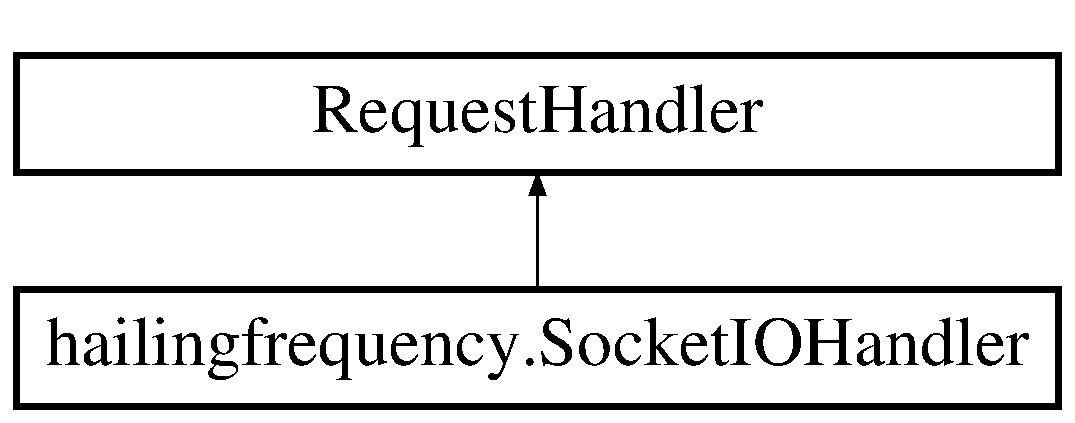
\includegraphics[height=2.000000cm]{classhailingfrequency_1_1_socket_i_o_handler}
\end{center}
\end{figure}
\subsection*{Public Member Functions}
\begin{DoxyCompactItemize}
\item 
\hypertarget{classhailingfrequency_1_1_socket_i_o_handler_a344624a70ebaa23998ce598a0dedbdc7}{def {\bfseries get}}\label{classhailingfrequency_1_1_socket_i_o_handler_a344624a70ebaa23998ce598a0dedbdc7}

\end{DoxyCompactItemize}


The documentation for this class was generated from the following file\-:\begin{DoxyCompactItemize}
\item 
hailingfrequency.\-py\end{DoxyCompactItemize}

\hypertarget{class_canary_models_1_1_temperature_1_1_temperature}{\section{Canary\-Models.\-Temperature.\-Temperature Class Reference}
\label{class_canary_models_1_1_temperature_1_1_temperature}\index{Canary\-Models.\-Temperature.\-Temperature@{Canary\-Models.\-Temperature.\-Temperature}}
}
Inheritance diagram for Canary\-Models.\-Temperature.\-Temperature\-:\begin{figure}[H]
\begin{center}
\leavevmode
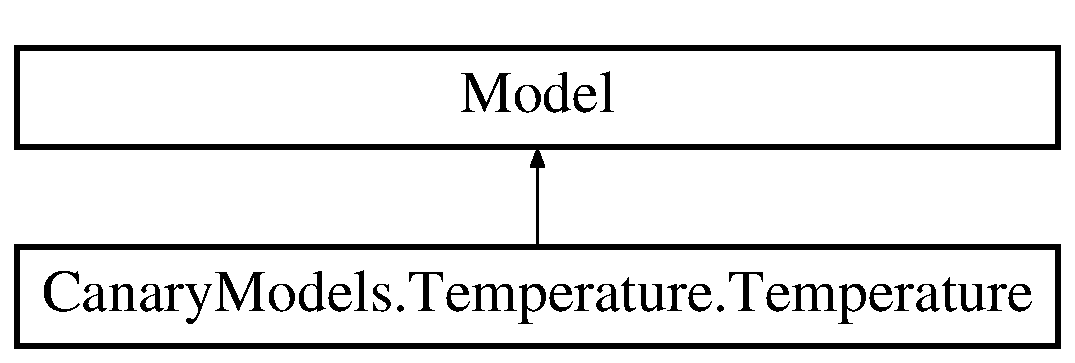
\includegraphics[height=2.000000cm]{class_canary_models_1_1_temperature_1_1_temperature}
\end{center}
\end{figure}
\subsection*{Public Member Functions}
\begin{DoxyCompactItemize}
\item 
\hypertarget{class_canary_models_1_1_temperature_1_1_temperature_a04dfdad3e16b916bd68850446510cdd2}{def {\bfseries \-\_\-\-\_\-init\-\_\-\-\_\-}}\label{class_canary_models_1_1_temperature_1_1_temperature_a04dfdad3e16b916bd68850446510cdd2}

\end{DoxyCompactItemize}


The documentation for this class was generated from the following file\-:\begin{DoxyCompactItemize}
\item 
Canary\-Models/Temperature.\-py\end{DoxyCompactItemize}

\hypertarget{class_canary_assets_1_1_user_1_1_user}{\section{Canary\-Assets.\-User.\-User Class Reference}
\label{class_canary_assets_1_1_user_1_1_user}\index{Canary\-Assets.\-User.\-User@{Canary\-Assets.\-User.\-User}}
}
Inheritance diagram for Canary\-Assets.\-User.\-User\-:\begin{figure}[H]
\begin{center}
\leavevmode
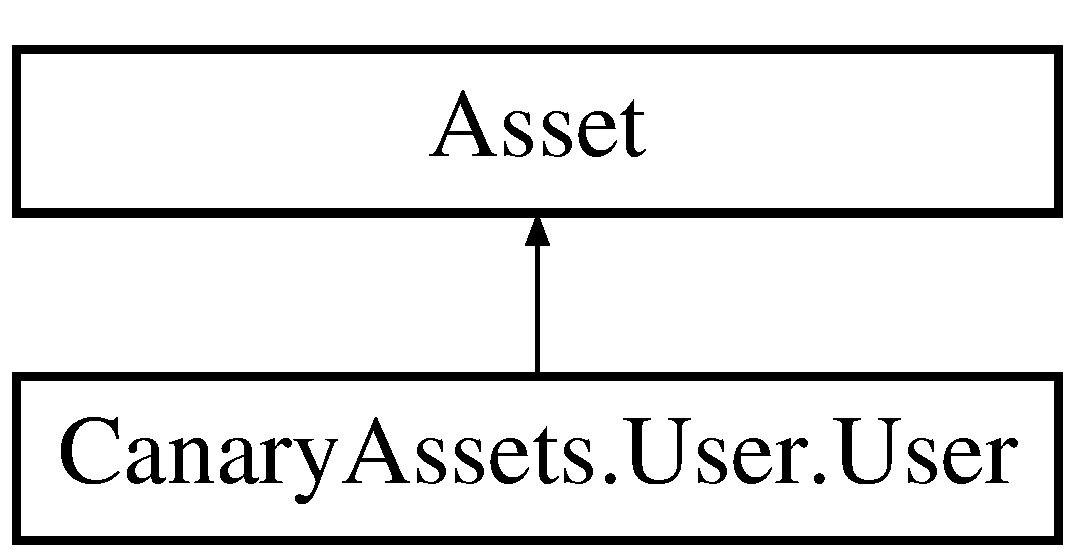
\includegraphics[height=2.000000cm]{class_canary_assets_1_1_user_1_1_user}
\end{center}
\end{figure}
\subsection*{Public Member Functions}
\begin{DoxyCompactItemize}
\item 
\hypertarget{class_canary_assets_1_1_user_1_1_user_af4ad306fd8dc77414541b293416f698c}{def {\bfseries \-\_\-\-\_\-init\-\_\-\-\_\-}}\label{class_canary_assets_1_1_user_1_1_user_af4ad306fd8dc77414541b293416f698c}

\item 
def \hyperlink{class_canary_assets_1_1_user_1_1_user_a1a73be79bd9c9360c51059ce7eaf2878}{add\-To\-Nest}
\item 
def \hyperlink{class_canary_assets_1_1_user_1_1_user_afa43d2b1b97ee68a8361c9e069eea374}{remove\-From\-Nest}
\end{DoxyCompactItemize}
\subsection*{Public Attributes}
\begin{DoxyCompactItemize}
\item 
\hypertarget{class_canary_assets_1_1_user_1_1_user_a488d6c32bf529e8a067285ce019aeca3}{{\bfseries nests}}\label{class_canary_assets_1_1_user_1_1_user_a488d6c32bf529e8a067285ce019aeca3}

\end{DoxyCompactItemize}


\subsection{Detailed Description}
\begin{DoxyVerb}The User class\end{DoxyVerb}
 

\subsection{Member Function Documentation}
\hypertarget{class_canary_assets_1_1_user_1_1_user_a1a73be79bd9c9360c51059ce7eaf2878}{\index{Canary\-Assets\-::\-User\-::\-User@{Canary\-Assets\-::\-User\-::\-User}!add\-To\-Nest@{add\-To\-Nest}}
\index{add\-To\-Nest@{add\-To\-Nest}!CanaryAssets::User::User@{Canary\-Assets\-::\-User\-::\-User}}
\subsubsection[{add\-To\-Nest}]{\setlength{\rightskip}{0pt plus 5cm}def Canary\-Assets.\-User.\-User.\-add\-To\-Nest (
\begin{DoxyParamCaption}
\item[{}]{self, }
\item[{}]{nest\-Id = {\ttfamily None}}
\end{DoxyParamCaption}
)}}\label{class_canary_assets_1_1_user_1_1_user_a1a73be79bd9c9360c51059ce7eaf2878}
\begin{DoxyVerb}Adds User to a Nest\end{DoxyVerb}
 \hypertarget{class_canary_assets_1_1_user_1_1_user_afa43d2b1b97ee68a8361c9e069eea374}{\index{Canary\-Assets\-::\-User\-::\-User@{Canary\-Assets\-::\-User\-::\-User}!remove\-From\-Nest@{remove\-From\-Nest}}
\index{remove\-From\-Nest@{remove\-From\-Nest}!CanaryAssets::User::User@{Canary\-Assets\-::\-User\-::\-User}}
\subsubsection[{remove\-From\-Nest}]{\setlength{\rightskip}{0pt plus 5cm}def Canary\-Assets.\-User.\-User.\-remove\-From\-Nest (
\begin{DoxyParamCaption}
\item[{}]{self, }
\item[{}]{nest\-Id = {\ttfamily None}}
\end{DoxyParamCaption}
)}}\label{class_canary_assets_1_1_user_1_1_user_afa43d2b1b97ee68a8361c9e069eea374}
\begin{DoxyVerb}Removes User from a Nest\end{DoxyVerb}
 

The documentation for this class was generated from the following file\-:\begin{DoxyCompactItemize}
\item 
Canary\-Assets/User.\-py\end{DoxyCompactItemize}

\hypertarget{classapi_1_1_user}{\section{api.\-User Class Reference}
\label{classapi_1_1_user}\index{api.\-User@{api.\-User}}
}
Inheritance diagram for api.\-User\-:\begin{figure}[H]
\begin{center}
\leavevmode
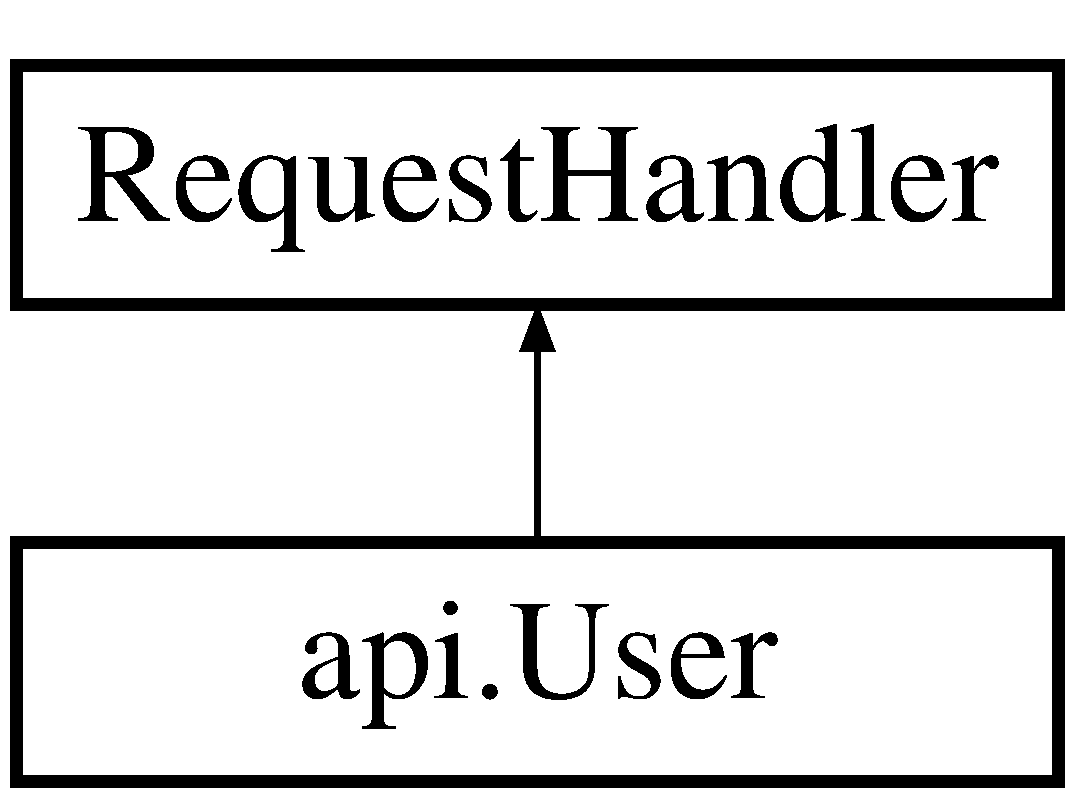
\includegraphics[height=2.000000cm]{classapi_1_1_user}
\end{center}
\end{figure}
\subsection*{Public Member Functions}
\begin{DoxyCompactItemize}
\item 
\hypertarget{classapi_1_1_user_a0f2cf0a3d4c5d606953358cb92a2b166}{def {\bfseries initialize}}\label{classapi_1_1_user_a0f2cf0a3d4c5d606953358cb92a2b166}

\item 
def \hyperlink{classapi_1_1_user_afd5bb645380fe6192ec6068fdcdda96e}{get}
\item 
def \hyperlink{classapi_1_1_user_a9365de26fbc9d590fce399ddf775a28f}{post}
\item 
def \hyperlink{classapi_1_1_user_aefffd1aa5d149b091f779b3222748fb5}{put}
\item 
def \hyperlink{classapi_1_1_user_a2868600f2d73a2e59e4a814205e5ae6e}{delete}
\end{DoxyCompactItemize}
\subsection*{Public Attributes}
\begin{DoxyCompactItemize}
\item 
\hypertarget{classapi_1_1_user_ad10ba6df28dbfe8546f24226c1ca28f6}{{\bfseries user\-Id}}\label{classapi_1_1_user_ad10ba6df28dbfe8546f24226c1ca28f6}

\end{DoxyCompactItemize}


\subsection{Member Function Documentation}
\hypertarget{classapi_1_1_user_a2868600f2d73a2e59e4a814205e5ae6e}{\index{api\-::\-User@{api\-::\-User}!delete@{delete}}
\index{delete@{delete}!api::User@{api\-::\-User}}
\subsubsection[{delete}]{\setlength{\rightskip}{0pt plus 5cm}def api.\-User.\-delete (
\begin{DoxyParamCaption}
\item[{}]{self, }
\item[{}]{nest\-Id}
\end{DoxyParamCaption}
)}}\label{classapi_1_1_user_a2868600f2d73a2e59e4a814205e5ae6e}
\begin{DoxyVerb}DELETE: deletes the User.\end{DoxyVerb}
 \hypertarget{classapi_1_1_user_afd5bb645380fe6192ec6068fdcdda96e}{\index{api\-::\-User@{api\-::\-User}!get@{get}}
\index{get@{get}!api::User@{api\-::\-User}}
\subsubsection[{get}]{\setlength{\rightskip}{0pt plus 5cm}def api.\-User.\-get (
\begin{DoxyParamCaption}
\item[{}]{self, }
\item[{}]{user\-Id}
\end{DoxyParamCaption}
)}}\label{classapi_1_1_user_afd5bb645380fe6192ec6068fdcdda96e}
\begin{DoxyVerb}GET: returns the User matching specified id.\end{DoxyVerb}
 \hypertarget{classapi_1_1_user_a9365de26fbc9d590fce399ddf775a28f}{\index{api\-::\-User@{api\-::\-User}!post@{post}}
\index{post@{post}!api::User@{api\-::\-User}}
\subsubsection[{post}]{\setlength{\rightskip}{0pt plus 5cm}def api.\-User.\-post (
\begin{DoxyParamCaption}
\item[{}]{self, }
\item[{}]{user\-Id}
\end{DoxyParamCaption}
)}}\label{classapi_1_1_user_a9365de26fbc9d590fce399ddf775a28f}
\begin{DoxyVerb}POST: log in/out the User matching specified id.\end{DoxyVerb}
 \hypertarget{classapi_1_1_user_aefffd1aa5d149b091f779b3222748fb5}{\index{api\-::\-User@{api\-::\-User}!put@{put}}
\index{put@{put}!api::User@{api\-::\-User}}
\subsubsection[{put}]{\setlength{\rightskip}{0pt plus 5cm}def api.\-User.\-put (
\begin{DoxyParamCaption}
\item[{}]{self, }
\item[{}]{user\-Id}
\end{DoxyParamCaption}
)}}\label{classapi_1_1_user_aefffd1aa5d149b091f779b3222748fb5}
\begin{DoxyVerb}PUT: updates the User's data.\end{DoxyVerb}
 

The documentation for this class was generated from the following file\-:\begin{DoxyCompactItemize}
\item 
api.\-py\end{DoxyCompactItemize}

\hypertarget{classapi_1_1_users}{\section{api.\-Users Class Reference}
\label{classapi_1_1_users}\index{api.\-Users@{api.\-Users}}
}
Inheritance diagram for api.\-Users\-:\begin{figure}[H]
\begin{center}
\leavevmode
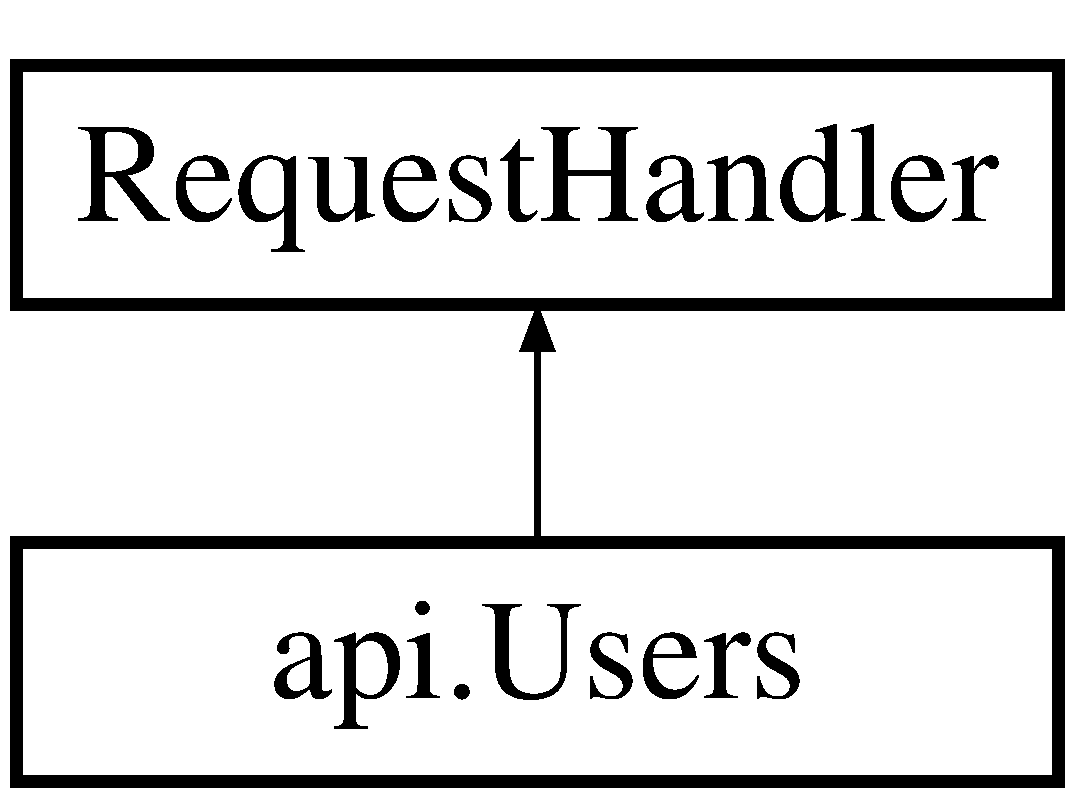
\includegraphics[height=2.000000cm]{classapi_1_1_users}
\end{center}
\end{figure}
\subsection*{Public Member Functions}
\begin{DoxyCompactItemize}
\item 
def \hyperlink{classapi_1_1_users_a5d177fece3eb6aa0e4bea1c5ddc07e36}{get}
\item 
def \hyperlink{classapi_1_1_users_a384872240d4628055a710f3082bfa356}{post}
\end{DoxyCompactItemize}


\subsection{Member Function Documentation}
\hypertarget{classapi_1_1_users_a5d177fece3eb6aa0e4bea1c5ddc07e36}{\index{api\-::\-Users@{api\-::\-Users}!get@{get}}
\index{get@{get}!api::Users@{api\-::\-Users}}
\subsubsection[{get}]{\setlength{\rightskip}{0pt plus 5cm}def api.\-Users.\-get (
\begin{DoxyParamCaption}
\item[{}]{self}
\end{DoxyParamCaption}
)}}\label{classapi_1_1_users_a5d177fece3eb6aa0e4bea1c5ddc07e36}
\begin{DoxyVerb}GET: returns a list of all Users [according to optional criteria].\end{DoxyVerb}
 \hypertarget{classapi_1_1_users_a384872240d4628055a710f3082bfa356}{\index{api\-::\-Users@{api\-::\-Users}!post@{post}}
\index{post@{post}!api::Users@{api\-::\-Users}}
\subsubsection[{post}]{\setlength{\rightskip}{0pt plus 5cm}def api.\-Users.\-post (
\begin{DoxyParamCaption}
\item[{}]{self}
\end{DoxyParamCaption}
)}}\label{classapi_1_1_users_a384872240d4628055a710f3082bfa356}
\begin{DoxyVerb}POST: creates a new User.

Post data must contain a valid User object.\end{DoxyVerb}
 

The documentation for this class was generated from the following file\-:\begin{DoxyCompactItemize}
\item 
api.\-py\end{DoxyCompactItemize}

%--- End generated contents ---

% Index
\newpage
\phantomsection
\addcontentsline{toc}{part}{Index}
\printindex

\end{document}
